% =============================================================================
% 商业智能大作业：基于深度神经网络的信用卡欺诈检测研究
% 编译器: XeLaTeX  |  文档类: ctexart
% =============================================================================

\documentclass[UTF8,a4paper,12pt,fontset=fandol]{ctexart}

% ── Packages ──────────────────────────────────────────────────────────
\usepackage{geometry}
\geometry{left=2.0cm,right=2.0cm,top=2.0cm,bottom=2.0cm}

\usepackage{graphicx}
\graphicspath{{figures/}}
\usepackage{booktabs}
\usepackage{hyperref}
\usepackage{amsmath,amssymb}
\usepackage{bm}
\usepackage{tikz}
\usetikzlibrary{positioning,arrows.meta,shapes,fit,backgrounds,calc}
\usepackage{algorithm2e}
\usepackage{float}
\usepackage{caption}
\usepackage{subcaption}
\usepackage{makecell}
\usepackage{array}
\usepackage{setspace}
\setstretch{1.05}
\setlength{\abovecaptionskip}{3pt}
\setlength{\belowcaptionskip}{3pt}
\setlength{\intextsep}{5pt plus 2pt minus 2pt}
\setlength{\textfloatsep}{5pt plus 2pt minus 2pt}

% Float page optimization — top-align so slack collects at bottom
\makeatletter
\setlength{\@fptop}{0pt}
\setlength{\@fpsep}{12pt}
\setlength{\@fpbot}{0pt plus 1fil}
\makeatother
\renewcommand{\topfraction}{0.90}
\renewcommand{\bottomfraction}{0.90}
\renewcommand{\textfraction}{0.07}
\renewcommand{\floatpagefraction}{0.75}

% ── References ────────────────────────────────────────────────────────
\usepackage[backend=biber,style=ieee,sorting=none]{biblatex}
\addbibresource{references.bib}

% ── Metadata ──────────────────────────────────────────────────────────
\title{\heiti\zihao{2} 深度神经网络在信用卡欺诈检测中的应用研究 \\
       \large ——基于树归纳偏置迁移的深度表格模型研究}
% \author{学生姓名 \\ 学号: XXXXXXXX}
\date{}

\begin{document}

\maketitle

% 中文摘要
\begin{abstract}
\noindent
信用卡欺诈检测是金融风控领域最具挑战性的问题之一，其类别高度不平衡的特性对机器学习方法提出了严峻考验。本文基于Kaggle 2023年信用卡欺诈检测数据集（56.8万条交易记录，经类别不平衡处理后使用约15万条样本），比较了两种异构深度神经网络架构（FT-Transformer、DeepFM）与XGBoost传统基线在欺诈检测任务上的表现，并提出了一种基于树归纳偏置迁移的知识蒸馏优化方案——将XGBoost的轴对齐分裂先验通过软标签蒸馏和特征重要性正则化迁移至深度模型。实验结果表明，DeepFM（AUPRC=0.9336）达到与XGBoost（0.9331）统计上不可区分的性能水平；FT-Transformer经Sparsemax替代Softmax后AUPRC达0.9179，且获得最低业务成本（Cost=99）。Tree-Supervised蒸馏消融实验揭示了一个关键的因果区分：软标签蒸馏（3A）在本研究条件下对两种架构均产生正向增益——FTT+KD达AUPRC=0.9347（+1.68pp）、DeepFM+KD达0.9495（+1.59pp），两者校准均近乎完美（ECE$<$0.001）；然而，特征重要性正则化（TreeReg, 3B）将FTT从0.9347大幅拖降至0.8974（-3.73pp），该效应与"树先验对嵌入层的刚性约束与Sparsemax注意力的自由交互学习存在结构性冲突"的假设一致，但替代解释（正则化强度不当、与KD的交互效应等）尚未完全排除。本文还结合SHAP分析、注意力可视化和商业成本矩阵，从可解释性和业务成本两个维度为模型选择提供实证依据。

\vspace{1em}
\noindent\textbf{关键词：}信用卡欺诈检测；深度神经网络；FT-Transformer；DeepFM；知识蒸馏；树归纳偏置；模型可解释性
\end{abstract}

% English Abstract
\begin{center}
{\Large\textbf{Abstract}}
\end{center}
\noindent
Credit card fraud detection remains one of the most challenging problems in financial risk management, where extreme class imbalance poses significant difficulties for standard classification approaches. This paper compares two heterogeneous deep neural network architectures (FT-Transformer and DeepFM) against the XGBoost baseline, and proposes a tree-supervised knowledge distillation method that transfers XGBoost's axis-aligned inductive bias to deep models via soft-label distillation and feature-importance regularization. Experiments use the Kaggle 2023 Credit Card Fraud Detection dataset comprising 568,000 transactions (approximately 150,000 after inducing realistic class imbalance). Results show that DeepFM (AUPRC=0.9336) achieves statistically indistinguishable performance from XGBoost (0.9331); FT-Transformer with Sparsemax achieves AUPRC=0.9179 after a +4.4pp improvement over Softmax. A critical ablation reveals that soft-label distillation (3A) benefits both architectures under the studied conditions — FTT+KD reaches AUPRC=0.9347 (+1.68pp), DeepFM+KD reaches 0.9495 (+1.59pp) — while feature-importance regularization (TreeReg, 3B) causes a substantial -3.73pp drop on FTT, consistent with a structural antagonism between tree-derived embedding constraints and self-attention, though alternative explanations (e.g., regularization strength, interaction with KD) remain to be excluded. Combined with SHAP analysis, attention visualization, and business cost matrices, this paper provides empirical evidence for model selection from both interpretability and cost perspectives.

\vspace{1em}
\noindent\textbf{Keywords:} Credit Card Fraud Detection; Deep Neural Networks; FT-Transformer; DeepFM; Knowledge Distillation; Tree Inductive Bias; Model Interpretability

% 引言章节

\section{引言}

\subsection{研究背景}

随着数字支付的普及，信用卡欺诈已成为全球金融体系面临的最严峻威胁之一。根据Nilson Report的最新数据，2023年全球信用卡欺诈损失预计超过350亿美元，且呈逐年增长趋势。传统的基于规则的风控系统在面对日益复杂的欺诈手段时显得力不从心——攻击者不断调整策略以规避固定规则，导致误报率居高不下，大量合法交易被误拦截，严重影响用户体验。

近年来，机器学习方法在欺诈检测领域展现出显著优势。相较于规则系统，机器学习模型能够自动从历史交易数据中学习欺诈模式，适应新型攻击手段。然而，欺诈检测面临一个根本性挑战：类别极端不平衡。在真实场景中，欺诈交易通常仅占总交易的0.1\%至1\%，这使得标准分类模型倾向于将所有交易预测为"正常"，从而导致欺诈漏检。

深度神经网络在计算机视觉和自然语言处理领域的成功引发了其在表格数据上的探索热潮。传统观点认为，梯度提升树（如XGBoost）在表格数据上的表现优于深度学习方法。但最新研究表明，专门为表格数据设计的深度架构——如FT-Transformer和DeepFM——在特定场景下能够接近甚至超越树模型。然而，深度模型在表格数据上的核心瓶颈并非模型容量，而是归纳偏置的错配：树模型的轴对齐分裂天然契合表格特征的异构性，而深度模型的全连接层和全局注意力缺乏这一先验。

\subsection{研究问题}

本文旨在回答以下核心研究问题：

\begin{enumerate}
    \item 深度表格模型（FT-Transformer、DeepFM）在信用卡欺诈检测任务上的表现是否能接近或超越XGBoost基线？自注意力机制和显式特征交互两种不同的归纳偏置在PCA匿名化特征空间中表现如何？
    \item 能否通过知识蒸馏将XGBoost的树归纳偏置（软标签分布 + 特征分裂重要性）迁移至深度模型，从而缩小深度模型与树模型之间的性能差距？
    \item 深度模型的注意力机制能否为欺诈检测提供有价值的可解释性？
    \item 在考虑实际业务成本的情况下，何种模型具有最佳的精度-成本权衡？
\end{enumerate}

\subsection{本文贡献}

本文的主要贡献如下：

\begin{enumerate}
    \item \textbf{统一评估框架下的异构架构横向比较}：在同一数据集和统一评估框架下，比较了两种异构深度表格架构（FT-Transformer的全局自注意力 vs. DeepFM的显式特征交互）与XGBoost基线的性能，揭示了不同归纳偏置在PCA匿名化特征空间中的表现差异；
    \item \textbf{树归纳偏置迁移方法}：提出了Tree-Supervised知识蒸馏方案，将XGBoost的软标签分布（方案3A）和特征分裂重要性先验（方案3B）迁移至FT-Transformer，验证了树模型的轴对齐归纳偏置可通过蒸馏增强深度模型的表格数据处理能力；
    \item \textbf{多维可解释性分析}：结合SHAP全局特征归因、个体瀑布图和FT-Transformer注意力权重，从多个视角解读模型决策逻辑，并诊断了自注意力在PCA空间中的均匀塌缩问题；
    \item \textbf{成本敏感评估}：引入业务成本矩阵（$C_{FP}=1$, $C_{FN}=10$），揭示AUPRC最优与业务成本最优之间的非单调关系，为实际部署提供帕累托前沿分析。
\end{enumerate}

\subsection{论文结构}

本文的其余部分组织如下：第二节回顾相关工作；第三节描述方法论；第四节呈现实验结果；第五节进行多维分析（可解释性、校准、成本）；第六节讨论商业启示、局限性和未来工作；第七节总结全文。

% 相关工作章节

\section{相关工作}

\subsection{传统信用卡欺诈检测方法}

信用卡欺诈检测的早期工作主要依赖基于规则的风控引擎和传统统计方法。逻辑回归（Logistic Regression）因其简单性和可解释性被广泛使用，但其线性假设限制了捕捉复杂欺诈模式的能力。决策树和随机森林（Random Forest）通过集成多棵决策树提升了泛化能力，并能处理非线性关系。Bhattacharyya等人\cite{bhattacharyya2011data}比较了支持向量机（SVM）、随机森林和逻辑回归在欺诈检测上的表现，发现随机森林在精确率-召回率权衡上表现最佳。

\subsection{梯度提升方法}

梯度提升树（Gradient Boosting Decision Trees）已成为表格数据上的标杆方法。XGBoost\cite{chen2016xgboost}通过引入正则化项和列采样防止过拟合，在多个Kaggle欺诈检测竞赛中占据主导地位。LightGBM和CatBoost进一步优化了训练效率和类别特征处理。然而，这些模型在处理极高维稀疏特征和复杂特征交互时仍存在局限，且缺乏对特征重要性的细粒度解释。

\subsection{深度表格模型}

近年来，研究者开始探索将深度学习应用于表格数据的有效方法。Borisov等人\cite{borisov2024deep}在其综述中系统性地梳理了表格深度学习的两大技术路线：基于Transformer的架构（如FT-Transformer、SAINT）和基于显式特征交互的架构（如DeepFM、DCN-V2），并指出表格数据对深度学习的独特挑战——异构特征、缺失值、不规则分布以及缺乏旋转不变性等归纳偏置。以下概述与本论文直接相关的代表性工作。

\textbf{FT-Transformer}\cite{gorishniy2021revisiting}将Transformer架构适配到表格数据。核心思想是将每个数值特征通过Feature Tokenizer映射为嵌入向量，在所有特征令牌前添加一个可学习的CLS令牌，然后通过标准Transformer编码器进行自注意力计算。CLS令牌的最终表示用于分类。FT-Transformer在多个表格数据基准上取得了有竞争力的结果，但在中等规模数据上树模型仍可能保持优势\cite{grinsztajn2022tree}。

\textbf{DeepFM}\cite{guo2017deepfm}结合了因子分解机（Factorization Machine）和深度神经网络。FM组件通过嵌入向量的内积高效捕获二阶特征交互，Deep组件通过多层感知机学习高阶特征表示。两者共享特征嵌入层，实现端到端联合训练。DeepFM最初用于点击率预测，但其特征交互建模能力同样适用于欺诈检测。

\textbf{SAINT}\cite{somepalli2022saint}在FT-Transformer的基础上引入了两种注意力机制的混合——对特征令牌间的自注意力（列注意力）和对样本间的行注意力——并通过自监督对比预训练提升了小样本场景下的性能。SAINT的结构设计表明，注意力机制的双重应用是表格深度学习的重要方向。

\subsection{后FT-Transformer时代：2022--2025年进展}

尽管FT-Transformer在多个基准上取得了优异表现，Grinsztajn等人\cite{grinsztajn2022tree}在45个表格数据集上的大规模实证研究发现了一个重要反例：在中等规模数据（$<$10万样本）上，基于树的模型（尤其是XGBoost和随机森林）即使不经过超参数调优，仍然持续优于深度模型。该研究指出，树模型的轴对齐分裂策略天然契合表格数据缺乏旋转不变性的特点，而神经网络对无信息特征（随机噪声列）更为敏感，性能下降幅度显著更大。这一发现对深度表格模型的研究方向产生了深远影响。

TabPFN\cite{hollmann2023tabpfn}提出了范式性的突破：通过在数百万合成数据集上预训练一个Transformer，使其学会贝叶斯推理过程，从而能在0.1秒内对新的小规模表格分类问题（$\le$1000样本、$\le$100特征）做出预测，且无需任何训练。但TabPFN目前受限于输入维度和小样本规模，尚无法直接应用于信用卡欺诈检测这类大规模场景。

Dastidar等人\cite{dastidar2024survey}在信用卡欺诈检测领域对机器学习和深度学习方法进行了系统综述，发现深度模型（尤其是LSTM和自编码器）在高维特征建模和序列行为检测方面具有独特优势，但在实际部署中仍面临数据隐私、类别不平衡和概念漂移等核心挑战。该综述进一步强调了AUPRC而非ROC-AUC作为主要评估指标的合理性，以及将可解释性分析纳入模型开发流程的必要性。

综上所述，本文的研究定位如下：在15万+样本的信用卡欺诈数据集上，以FT-Transformer（全局自注意力）和DeepFM（显式特征交互）代表两种不同的归纳偏置，系统比较深度表格模型与传统梯度提升方法在AUPRC和商业成本指标上的表现。在此基础上，本文引入Tree-Supervised知识蒸馏方案，将XGBoost的树结构先验迁移至深度模型，探索"以树为师"的归纳偏置增强路径。同时，通过SHAP分析和注意力可视化，为不平衡学习和可解释性提供实证证据。

\subsection{类别不平衡处理}

针对类别不平衡问题，现有方法可分为三大类：（1）数据层面方法，如随机过采样和SMOTE\cite{chawla2002smote}，通过生成少数类合成样本来平衡训练集；（2）算法层面方法，如类别加权和代价敏感学习，通过调整损失函数中不同类别的权重来关注少数类；（3）损失函数改进，如Focal Loss\cite{lin2017focal}，通过降低易分类样本的损失贡献，使模型聚焦于难分类样本。本文在实验部分对这三类方法进行了系统比较。

\subsection{模型可解释性}

在金融风控场景中，模型可解释性不仅是监管合规的要求，更是获取业务方信任的关键。SHAP\cite{lundberg2017unified}基于Shapley值的博弈论框架，为每个特征分配对预测结果的贡献值，是目前最被广泛接受的可解释性方法之一。对于树模型，TreeExplainer提供了快速精确的SHAP值计算。对于深度模型，FT-Transformer的内置注意力机制提供了额外的可解释性维度——通过可视化[CLS] Token对各特征的注意力权重，可以直观理解模型在做出预测时关注了哪些特征。

% 方法论章节

\section{方法论}

\subsection{符号定义}

为保持全文符号一致性，本文采用以下统一符号体系：

\begin{table}[H]
\centering
\caption{全文统一符号定义。包含数据集、特征向量、类别标签、模型预测函数、分类阈值、混淆矩阵元素和业务成本等核心符号。}
\label{tab:notation}
\begin{tabular}{cl}
\toprule
\textbf{符号} & \textbf{含义} \\
\midrule
$\mathcal{D}$ & 完整数据集 $\mathcal{D} = \{(\mathbf{x}_i, y_i)\}_{i=1}^{N}$ \\
$\mathbf{x}_i \in \mathbb{R}^d$ & 第$i$个样本的特征向量（$d=29$） \\
$y_i \in \{0, 1\}$ & 类别标签（$0$=正常交易，$1$=欺诈交易） \\
$\mathcal{D}_{\text{train}}, \mathcal{D}_{\text{val}}, \mathcal{D}_{\text{test}}$ & 训练集、验证集、测试集 \\
$N$ & 样本总数 \\
$d$ & 特征维度 \\
$f(\cdot)$ & 模型预测函数，$f: \mathbb{R}^d \to [0, 1]$ \\
$\hat{y}_i = f(\mathbf{x}_i)$ & 模型对样本$i$的预测概率 \\
$\tau$ & 分类阈值，$\hat{y}_i \geq \tau$ 判定为欺诈 \\
TP, FP, FN, TN & 真正例、假正例、假负例、真负例 \\
$\text{Cost}$ & 业务成本，$\text{Cost} = C_{FP} \cdot \text{FP} + C_{FN} \cdot \text{FN}$ \\
$C_{FP}, C_{FN}$ & 误报成本、漏报成本（$C_{FP}=1, C_{FN}=10$） \\
$\phi_j$ & 特征$j$的Shapley值 \\
\bottomrule
\end{tabular}
\end{table}

\subsection{数据来源与探索性分析}

本文采用Kaggle平台上的Credit Card Fraud Detection Dataset 2023数据集\cite{kaggle2023fraud}。该数据集包含信用卡交易记录，原始数据超过56.8万条，且正负类接近1:1平衡。然而，真实信用卡欺诈的比率通常仅为0.1\%--1\%，为模拟这一现实场景，本文对多数类（正常交易）进行下采样并限制最大样本数为150,000，同时从少数类（欺诈交易）中随机抽取750条，使最终欺诈比例约为0.5\%（正负比约1:200）。数据已通过PCA进行部分匿名化处理，但其规模（处理后150,750条记录）为深度学习模型提供了充足的训练样本。

\subsubsection{数据集特征}

数据集共包含31个特征列：28个匿名化PCA特征（V1-V28）、交易金额（Amount）和类别标签（Class，0=正常，1=欺诈）。初步探索性分析显示：

\begin{itemize}
    \item 总交易数：150,750（150,000正常 + 750欺诈）
    \item 欺诈交易占比：0.5\%（严重不平衡，正负比约1:200）
    \item 无缺失值，所有特征均为数值型
    \item Amount特征呈现典型的长尾分布
    \item 部分V特征在欺诈和正常交易间呈现显著分布差异
\end{itemize}

图\ref{fig:class_balance}呈现了经不平衡处理后的完整数据集类别分布：正常交易样本数为150,000，欺诈交易样本数仅为750，正负类比例约为200:1。这种极端的类别不平衡是信用卡欺诈检测任务的核心挑战——模型在训练过程中极易被多数类主导，导致对少数类的识别能力严重退化。仅0.5\%的欺诈比例意味着，即使一个"将所有交易预测为正常"的朴素分类器也能达到99.5\%的准确率——这正是准确率（Accuracy）在不平衡场景下完全失效的原因，也解释了本文为何采用AUPRC而非准确率作为主要评估指标。

图\ref{fig:amount_dist}以核密度估计对比了两类交易的金额分布。蓝色曲线（正常交易，$n=150,000$）和橙色曲线（欺诈交易，$n=750$）均呈现明显的右偏（长尾）分布，但存在两个关键差异：第一，欺诈交易的KDE峰值位置略高于正常交易，表明欺诈者倾向于选择中等偏高的交易金额以在"隐匿性"与"收益"之间取得平衡；第二，在高金额区间（$>15,000$标准化单位），欺诈交易的密度相对更高，这与银行业务经验一致——高价值交易是欺诈者的优先目标。然而，两类分布在整体上存在大量重叠区域，意味着仅凭交易金额远不足以区分欺诈与正常交易，必须依赖多维特征联合判别。

\begin{figure}[htbp]
    \centering
    
\includegraphics[width=0.75\textwidth]{class_balance.pdf}
    \caption{经不平衡处理后的数据集类别分布。正常交易150,000条，欺诈交易750条，正负比约200:1，准确率在此场景下完全失效。}
    \label{fig:class_balance}
\end{figure}

\begin{figure}[htbp]
    \centering
    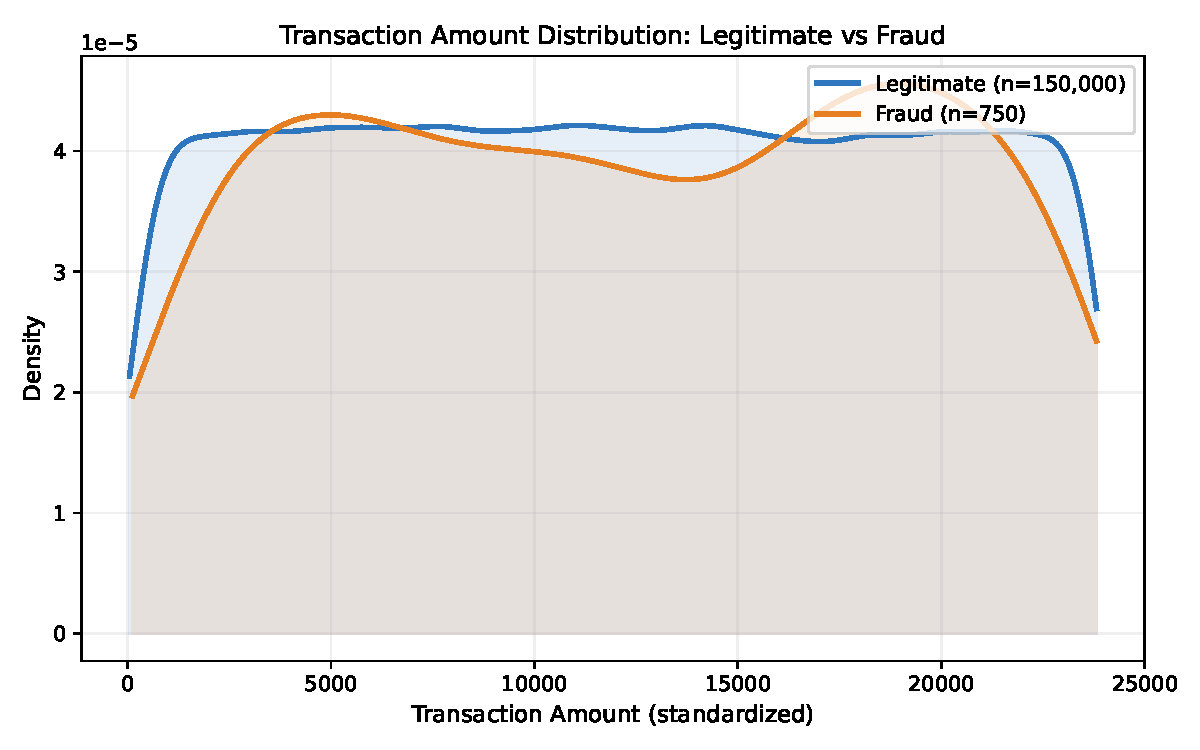
\includegraphics[width=0.78\textwidth]{amount_distribution.pdf}
    \caption{正常交易与欺诈交易的金额核密度估计曲线。蓝色为正常交易，橙色为欺诈交易，两类均呈右偏分布且存在大量重叠，欺诈交易在高金额区间密度略高。}
    \label{fig:amount_dist}
\end{figure}

上述EDA结果表明，任何有效的欺诈检测模型必须：（1）采用针对性的不平衡处理策略（如Focal Loss、SMOTE或类别加权），因为0.5\%的欺诈率使标准分类器失效；（2）依赖多特征联合判别而非单一金额阈值，因为两类金额分布存在大量重叠；（3）在评估时优先使用对类别不平衡敏感的指标（如AUPRC而非ROC-AUC或准确率）。

\subsection{数据预处理}

数据预处理流水线包含以下步骤：

\begin{enumerate}
    \item \textbf{特征选择}：移除ID列（不携带预测信息）。
    \item \textbf{异常值处理}：对Amount特征采用IQR方法进行异常值截断（仅在训练集上计算上下界，避免数据泄露）。V1-V28为PCA变换后的特征，其分布为原始特征的线性组合，不具有传统意义上的"异常值"含义，因此不做截断处理。
    \item \textbf{标准化}：使用StandardScaler对所有数值特征进行标准化（拟合于训练集，应用于验证集和测试集）。
    \item \textbf{数据集划分}：按70\%/15\%/15\%进行分层划分（Stratified Split），确保各个子集中欺诈比例一致。
\end{enumerate}

\subsection{模型架构}

本文实现并比较了两种异构深度神经网络架构与XGBoost传统基线。在此基础上，引入Tree-Supervised知识蒸馏方案（第三节），将XGBoost的树归纳偏置迁移至FT-Transformer：

\subsubsection{XGBoost基线}

XGBoost（eXtreme Gradient Boosting）\cite{chen2016xgboost}作为传统表格数据的强基线，采用梯度提升树框架。本文使用300轮提升、最大深度8、学习率0.05，并通过scale\_pos\_weight参数根据训练集正负比自动调节类别权重。为充分利用数据，XGBoost在训练集和验证集的合并数据上训练。

% =============================================================================
% FT-Transformer 原理深度讲解
% =============================================================================

\subsection{FT-Transformer：特征令牌化与自注意力机制}

FT-Transformer（Feature Tokenizer + Transformer）由Gorishniy等人\cite{gorishniy2021revisiting}于2021年提出，其核心思想是将表格数据的每个数值特征视为一个独立的"词元"（Token），通过Transformer编码器的自注意力机制学习特征间的全局交互。以下从四个层面逐层拆解其工作原理。

\subsubsection{整体架构}

FT-Transformer将表格分类问题转化为类似NLP的序列分类问题：每条数据记录被表示为一个特征令牌序列，模型通过在所有特征上计算成对注意力来捕获特征间关系。图\ref{fig:ftt_arch}以流程图呈现了从原始特征到最终预测的完整数据流。

\begin{figure}[htbp]
\centering
\begin{tikzpicture}[
    node distance=0.5cm,
    box/.style={rectangle, draw=black!70, rounded corners=3pt, minimum width=5.0cm, minimum height=0.62cm, align=center, font=\footnotesize},
    smallbox/.style={rectangle, draw=black!50, rounded corners=2pt, minimum width=2.2cm, minimum height=0.55cm, align=center, font=\scriptsize},
    arrow/.style={-{Stealth[scale=1.0]}, thick, black!60},
]
    % Main flow
    \node[box, fill=blue!5] (input) {输入 $\mathbf{x} = [x_1, \dots, x_{29}] \in \mathbb{R}^{29}$};
    \node[box, fill=blue!8, below=of input] (tokenizer) {Feature Tokenizer: $T_j = x_j \cdot \bm{W}_j + \bm{b}_j$ \quad ($\bm{W}_j,\bm{b}_j \in \mathbb{R}^{64}$)};
    \node[box, fill=green!5, below=of tokenizer] (cls) {前置 [CLS]: $\mathbf{Z} = [T_{\mathrm{CLS}}, T_1, \dots, T_{29}] \in \mathbb{R}^{30 \times 64}$};
    \node[box, fill=orange!8, below=of cls] (encoder) {Transformer Encoder $\times 3$\\(多头自注意力 + FFN + 残差连接 + LayerNorm)};
    \node[box, fill=green!5, below=of encoder] (extract) {提取 [CLS] 表示: $\mathbf{h}_{\mathrm{CLS}}^{(3)} \in \mathbb{R}^{64}$};
    \node[box, fill=red!5, below=of extract] (head) {LayerNorm $\to$ Linear($64{\to}1$) $\to$ Sigmoid};
    \node[box, fill=red!8, below=of head] (output) {输出: $\hat{y} \in [0, 1]$ （欺诈概率）};

    % Arrows
    \draw[arrow] (input) -- (tokenizer);
    \draw[arrow] (tokenizer) -- (cls);
    \draw[arrow] (cls) -- (encoder);
    \draw[arrow] (encoder) -- (extract);
    \draw[arrow] (extract) -- (head);
    \draw[arrow] (head) -- (output);

    % Encoder detail callout
    \node[smallbox, fill=orange!15, right=2.2cm of encoder] (attn) {Multi-Head\\Self-Attention};
    \node[smallbox, fill=orange!15, right=2.2cm of attn] (ffn) {Feed-Forward\\Network};
    \draw[arrow, dashed, orange!70] (encoder.east) -- ++(0.4,0) |- (attn.west);
    \draw[arrow, dashed, orange!70] (encoder.east) -- ++(0.4,0) |- (ffn.west);
\end{tikzpicture}
\caption{FT-Transformer架构流程图。29个数值特征经Feature Tokenizer映射为64维嵌入向量，前置可学习的[CLS] Token后送入3层Transformer编码器。[CLS]的最终输出经LayerNorm和线性层得到欺诈概率。右侧虚线框展示编码器内部两大核心组件。}
\label{fig:ftt_arch}
\end{figure}

\subsubsection{第一层：Feature Tokenizer——为什么数值需要"嵌入"}

传统做法将表格数据的一行直接输入MLP（$\mathbb{R}^{29} \to \text{Linear}(29, 64)$），这等价于对所有特征使用同一个投影矩阵。FT-Transformer的关键创新在于为每个特征$j$分配独立的可学习参数$\bm{W}_j$和$\bm{b}_j$：

\begin{equation}
T_j = x_j \cdot \bm{W}_j + \bm{b}_j \in \mathbb{R}^{d_{model}}
\label{eq:tokenize}
\end{equation}

其中$\bm{W}_j$的作用不是线性变换（因为$x_j$是标量），而是\textbf{特征专属的嵌入向量}——将标量特征值沿特定方向"拉伸"为$d_{model}$维向量。理解这一设计的关键在于：

\begin{itemize}
    \item \textbf{异构特征需要异构空间}：V14（强判别性PCA成分）和V25（近噪声成分）的变化量$\Delta x$对最终决策的影响截然不同。若所有特征共享同一投影矩阵，模型将无法区分"重要的0.1"和"不重要的0.1"。Feature Tokenizer使每个特征拥有独立的"语义通道"，其嵌入向量的方向编码了该特征的身份（identity），模长编码了其数值强度。
    \item \textbf{为注意力提供可区分的Key/Query}：自注意力通过Query-Key内积$\langle \bm{Q}_i, \bm{K}_j \rangle$度量特征$i$对特征$j$的"关注程度"。若特征嵌入是同一线性变换的产物，则所有特征将位于同一低维子空间，Query-Key内积丧失区分度——这正是本文在PCA匿名化数据上观察到的"注意力均匀塌缩"的根本原因。
\end{itemize}

在本文的实验中，$d_{model}=64$意味着每个标量特征被映射为一个64维向量，29个特征共计产生$29 \times (64 + 64) = 3,\!712$个专属参数。

\subsubsection{第二层：[CLS] Token——从序列到分类的桥梁}

借鉴BERT \cite{devlin2018bert}的设计，FT-Transformer在所有特征令牌前添加一个可学习的[CLS] Token $T_{\mathrm{CLS}} \in \mathbb{R}^{d_{model}}$，形成长度为30的序列：

\begin{equation}
\mathbf{Z}_0 = [T_{\mathrm{CLS}}, T_1, T_2, \dots, T_{29}] \in \mathbb{R}^{30 \times 64}
\end{equation}

[CLS] Token的设计哲学是\textbf{信息汇聚}：它自身不携带任何特征信息（随机初始化），但在经过多层自注意力后，它通过Query机制从所有特征令牌中"抽取"了对分类最有用的信息。可以理解为——[CLS]是模型学会的"最佳问题"（optimal query），而每个特征令牌提供的是该特征的"回答"（key-value pair）。最终，仅[CLS]的输出被送入分类头，其余29个特征令牌的输出被丢弃。

\subsubsection{第三层：Multi-Head Self-Attention——特征间的全局对话}

这是FT-Transformer的核心计算引擎。给定输入序列$\mathbf{Z} \in \mathbb{R}^{S \times d}$（$S=30$），单头自注意力执行以下操作：

\textbf{Step 1：线性投影。}将每个令牌分别投影为Query、Key、Value三个向量：
\begin{equation}
\mathbf{Q} = \mathbf{Z}\mathbf{W}_Q,\quad \mathbf{K} = \mathbf{Z}\mathbf{W}_K,\quad \mathbf{V} = \mathbf{Z}\mathbf{W}_V
\end{equation}
其中$\mathbf{W}_Q, \mathbf{W}_K, \mathbf{W}_V \in \mathbb{R}^{d \times d_k}$，$d_k = d_{model} / n_{heads} = 8$。

\textbf{Step 2：Scaled Dot-Product Attention。}计算每对令牌间的注意力分数：
\begin{equation}
\mathrm{Attention}(\mathbf{Q}, \mathbf{K}, \mathbf{V}) = \mathrm{Sparsemax}\!\left(\frac{\mathbf{Q}\mathbf{K}^\top}{\sqrt{d_k}}\right) \mathbf{V}
\label{eq:attention}
\end{equation}

除以$\sqrt{d_k}$的目的是防止内积过大导致Sparsemax/Softmax饱和（梯度消失）。30个令牌的注意力矩阵为$\mathbb{R}^{30 \times 30}$——每个特征对其他29个特征（包括[CLS]和自身）分配一个注意力权重。

\textbf{Step 3：Multi-Head 整合。}并行执行$n_{heads}=8$个独立的注意力计算（每头使用不同的$\mathbf{W}_Q, \mathbf{W}_K, \mathbf{W}_V$），将各头输出拼接后线性投影：

\begin{equation}
\mathrm{MultiHead}(\mathbf{Z}) = \mathrm{Concat}(\mathrm{head}_1, \dots, \mathrm{head}_8) \mathbf{W}_O
\end{equation}

多头设计使模型能在不同的表示子空间中同时关注不同类型的关系——例如，一个头可能聚焦于V14-V12的相关性，另一个头关注V4-V17的交互。然而，本文的实验发现：在PCA匿名化特征上，各头输出的注意力分布高度相似，表明PCA破坏了供多头分化的语义多样性。

\textbf{Step 4：Transformer Encoder Block。}每个编码器层包含两个子层，每子层均有残差连接和LayerNorm：

\begin{equation}
\begin{aligned}
\mathbf{Z}' &= \mathrm{LayerNorm}\big(\mathbf{Z} + \mathrm{MultiHead}(\mathbf{Z})\big) \\
\mathbf{Z}'' &= \mathrm{LayerNorm}\big(\mathbf{Z}' + \mathrm{FFN}(\mathbf{Z}')\big)
\end{aligned}
\end{equation}

其中FFN为两层MLP：$\mathrm{FFN}(\mathbf{x}) = \mathrm{GELU}(\mathbf{x}\mathbf{W}_1 + \mathbf{b}_1)\mathbf{W}_2 + \mathbf{b}_2$，中间维度$d_{ffn}=256$提供4倍于$d_{model}$的容量以进行非线性变换。残差连接确保即使注意力学不到有用信息（如均匀塌缩），梯度仍能通过恒等路径回传，避免深层网络的退化。

\subsubsection{第四层：Sparsemax——本文的关键改进}

原始FT-Transformer使用Softmax归一化注意力权重：
\begin{equation}
\mathrm{Softmax}(\mathbf{z})_i = \frac{e^{z_i}}{\sum_j e^{z_j}}
\end{equation}

Softmax存在两个固有问题：（1）它永远输出全非零的概率分布（$e^{z_i} > 0$恒成立），无法产生真正的稀疏解；（2）当所有$z_i$接近时（如在PCA空间中），输出趋于均匀分布$1/d$。

本文采用Sparsemax \cite{martins2016sparsemax}替代Softmax。Sparsemax将logits向量$\mathbf{z}$投影到概率单纯形（probability simplex）上，产生\textbf{可能包含零值}的稀疏概率分布：

\begin{equation}
\mathrm{Sparsemax}(\mathbf{z}) = \arg\min_{\mathbf{p} \in \Delta^{d-1}} \|\mathbf{p} - \mathbf{z}\|_2^2
\end{equation}

其闭式解为$\mathrm{Sparsemax}(\mathbf{z})_i = \max(z_i - \tau(\mathbf{z}), 0)$，其中$\tau(\mathbf{z})$是确保$\sum_i \max(z_i - \tau, 0) = 1$的唯一阈值。算法复杂度为$O(d \log d)$，不增加计算负担。

\textbf{核心差异}：Softmax对低logits值赋予微量但非零的概率（如0.001），Sparsemax直接将其设为零。在表格数据语境中，这意味着特征$j$完全可以被排除在特征$i$的"注意力视野"之外——模型被强制做出选择。本实验证实，Sparsemax将FT-Transformer的AUPRC从0.8738提升至0.9179（+4.4pp），ECE从0.2328降至0.0120（改善约20倍）。

需要指出，本文未分离Sparsemax的稀疏化效应与其隐式的温度/熵调节效应——Sparsemax的投影操作（$\ell_2$范数最小化至单纯形）在降低输出熵的同时引入稀疏性，两者可能独立贡献于AUPRC和ECE的改善。Softmax+温度缩放（temperature scaling）可能以不同机制实现类似的熵调节效果，这一替代路径留待未来验证。

\subsubsection{本文配置与训练细节}

\begin{itemize}
    \item $d_{model}=64, n_{heads}=8, n_{layers}=3, d_{ffn}=256$
    \item 总参数量：153,921（合理范围，避免过拟合15万训练样本）
    \item 优化器：AdamW（lr=$5 \times 10^{-4}$, weight\_decay=$10^{-4}$）
    \item 损失函数：Focal Loss（$\alpha=0.25, \gamma=2.0$）——$\alpha=0.25$被选为Sparsemax的搭配，因稀疏注意力需要均衡的正负类梯度信号
    \item 早停：验证集AUPRC连续15轮不提升
\end{itemize}

% =============================================================================
% DeepFM 原理深度讲解
% =============================================================================

\subsection{DeepFM：显式特征交互与因子分解机}

DeepFM由Guo等人\cite{guo2017deepfm}于2017年提出，最初应用于点击率（CTR）预测。其核心思想是将因子分解机（Factorization Machine, FM）的显式二阶特征交互与深度神经网络的高阶表示学习融合于一个端到端框架中。与FT-Transformer的"隐式"交互（通过注意力权重间接建模）不同，DeepFM采用"显式"交互——直接计算每对特征的向量内积。

\subsubsection{整体架构}

DeepFM由三个组件构成，共享底层的特征嵌入层。图\ref{fig:deepfm_arch}展示了从前向传播到最终预测的完整数据流。

\begin{figure}[htbp]
\centering
\begin{tikzpicture}[
    node distance=0.5cm,
    box/.style={rectangle, draw=black!70, rounded corners=3pt, minimum width=5.4cm, minimum height=0.6cm, align=center, font=\footnotesize},
    branch/.style={rectangle, draw=black!50, rounded corners=2pt, minimum width=2.6cm, minimum height=0.58cm, align=center, font=\scriptsize},
    arrow/.style={-{Stealth[scale=1.0]}, thick, black!60},
    merge/.style={circle, draw=black!70, fill=black!5, minimum size=0.55cm, font=\small},
]
    % Main flow
    \node[box, fill=blue!5] (input) {输入 $\mathbf{x} = [x_1, \dots, x_{29}] \in \mathbb{R}^{29}$};
    \node[box, fill=green!8, below=of input] (embed) {共享嵌入: $\mathbf{e}_i = x_i \cdot \mathbf{v}_i \in \mathbb{R}^{16}$ ($i = 1,\dots,29$)};
    \node[box, fill=orange!5, below=0.15cm of embed] (split) {分两路：FM路径 + Deep路径（共享嵌入参数）};

    % FM branch
    \node[branch, fill=yellow!8, below left=0.6cm and -1.6cm of split] (linear) {一阶线性: $\sum_{i} w_i x_i$};
    \node[branch, fill=yellow!8, below=0.3cm of linear] (second) {二阶交互: $\sum_{i<j}\langle\mathbf{v}_i,\mathbf{v}_j\rangle x_i x_j$};

    % Deep branch
    \node[branch, fill=cyan!8, below right=0.6cm and -1.6cm of split] (dense1) {Dense(464$\to$256) + ReLU};
    \node[branch, fill=cyan!8, below=0.3cm of dense1] (dense2) {Dense(256$\to$128) + ReLU};
    \node[branch, fill=cyan!8, below=0.3cm of dense2] (dense3) {Dense(128$\to$64) + ReLU};

    % Merge
    \node[merge, below=2.0cm of split] (merge) {$\Sigma$};
    \node[box, fill=red!5, below=0.35cm of merge] (sigmoid) {$\sigma\!\left(w_0 + \text{FM} + \text{Deep}\right)$};
    \node[box, fill=red!8, below=0.35cm of sigmoid] (output) {输出: $\hat{y} \in [0, 1]$};

    % Arrows from input
    \draw[arrow] (input) -- (embed);
    \draw[arrow] (embed) -- (split);

    % FM branch arrows
    \draw[arrow] (split.south) -- ++(0, -0.25) -| (linear.north);
    \draw[arrow] (linear) -- (second);
    \draw[arrow] (second.south) -- ++(0, -0.2) -| (merge.west);

    % Deep branch arrows
    \draw[arrow] (split.south) -- ++(0, -0.25) -| (dense1.north);
    \draw[arrow] (dense1) -- (dense2);
    \draw[arrow] (dense2) -- (dense3);
    \draw[arrow] (dense3.south) -- ++(0, -0.2) -| (merge.east);

    % Merge to output
    \draw[arrow] (merge) -- (sigmoid);
    \draw[arrow] (sigmoid) -- (output);

    % Annotation
    \node[font=\scriptsize\itshape, black!45, right=1.0cm of second] {FM: $O(DK)$};
    \node[font=\scriptsize\itshape, black!45, right=1.0cm of dense3] {Deep: MLP};
\end{tikzpicture}
\caption{DeepFM架构流程图。29个数值特征经共享嵌入层映射为16维向量，分两路并行计算：FM路径执行显式一阶和二阶特征交互，Deep路径通过三层MLP学习高阶表示。两路输出与全局偏置$w_0$求和后经Sigmoid输出。共享嵌入是DeepFM的核心设计——FM的交互质量直接影响Deep路径的初始表示。}
\label{fig:deepfm_arch}
\end{figure}

\subsubsection{第一层：共享嵌入}

每个特征$x_i$（标量）被映射为一个$K$维嵌入向量（本文$K=16$）：

\begin{equation}
\mathbf{e}_i = x_i \cdot \mathbf{v}_i \in \mathbb{R}^{K}
\label{eq:deepfm_embed}
\end{equation}

其中$\mathbf{v}_i \in \mathbb{R}^{K}$是特征$i$的专属嵌入向量。所有这些$\mathbf{v}_i$在FM组件和Deep组件之间\textbf{共享}——这意味着FM学习到的成对关系会通过反向传播同时优化Deep路径使用的嵌入表示。共享机制是DeepFM超越"FM+MLP串联"的关键：两个组件的训练信号在嵌入层交汇，FM提供的结构化交互信号充当Deep路径的正则化先验。

\subsubsection{第二层：FM组件}

FM组件由两部分组成：

\textbf{一阶部分（线性）：}
\begin{equation}
y_{\mathrm{linear}} = w_0 + \sum_{i=1}^{D} w_i x_i
\end{equation}

这部分等价于逻辑回归——每个特征有独立的线性权重$w_i$，直接对预测值做加减。$w_0$是全局偏置。

\textbf{二阶部分（成对交互）：}
\begin{equation}
y_{\mathrm{FM}} = \sum_{i=1}^{D} \sum_{j=i+1}^{D} \langle \mathbf{v}_i, \mathbf{v}_j \rangle \cdot x_i x_j
\label{eq:fm_interaction}
\end{equation}

这是FM的核心。对每一对特征$(i, j)$，其交互强度由两个因素共同决定：
\begin{enumerate}
    \item \textbf{数值乘积} $x_i \cdot x_j$：如果两个特征同时偏高（如V14和V12均异常高），乘积大→交互贡献大。
    \item \textbf{嵌入相似度} $\langle \mathbf{v}_i, \mathbf{v}_j \rangle$：两个特征的嵌入向量越"对齐"（内积越大），它们对预测的协同效应越强。
\end{enumerate}

\textbf{关键数学技巧——$O(D^2K) \to O(DK)$：}直接计算公式\eqref{eq:fm_interaction}需要对$D(D-1)/2$对特征各计算一次$K$维内积，复杂度$O(D^2K)$。通过以下代数变换可降至$O(DK)$：

\begin{equation}
\begin{aligned}
\sum_{i=1}^{D}\sum_{j=i+1}^{D} \langle \mathbf{v}_i, \mathbf{v}_j \rangle x_i x_j
&= \frac{1}{2}\left(\sum_{i=1}^{D}\sum_{j=1}^{D} \langle \mathbf{v}_i, \mathbf{v}_j \rangle x_i x_j - \sum_{i=1}^{D} \langle \mathbf{v}_i, \mathbf{v}_i \rangle x_i^2 \right) \\
&= \frac{1}{2}\left( \sum_{f=1}^{K}\left(\sum_{i=1}^{D} v_{i,f} x_i\right)^2 - \sum_{i=1}^{D}\sum_{f=1}^{K} v_{i,f}^2 x_i^2 \right)
\end{aligned}
\label{eq:fm_trick}
\end{equation}

式\eqref{eq:fm_trick}的关键在于将双重求和$\sum_i\sum_j$转化为先对$i$求和再平方的结构——这只需要$O(DK)$次乘法和加法，而非$O(D^2K)$次。当$D=29$时，$O(DK)=464$次操作 vs. $O(D^2K)=13,456$次操作，加速约29倍。这一变换使得FM的大规模特征交互在计算上可行。

\subsubsection{第三层：Deep组件}

Deep组件是一个标准的前馈神经网络，接收所有特征嵌入向量的拼接（flatten）作为输入：

\begin{equation}
\mathbf{h}_0 = \mathrm{Concat}(\mathbf{e}_1, \mathbf{e}_2, \dots, \mathbf{e}_{29}) \in \mathbb{R}^{D \times K = 464}
\end{equation}

随后通过三层全连接网络：

\begin{equation}
\begin{aligned}
\mathbf{h}_1 &= \mathrm{ReLU}(\mathbf{W}_1 \mathbf{h}_0 + \mathbf{b}_1), \quad \mathbf{W}_1 \in \mathbb{R}^{256 \times 464} \\
\mathbf{h}_2 &= \mathrm{ReLU}(\mathbf{W}_2 \mathbf{h}_1 + \mathbf{b}_2), \quad \mathbf{W}_2 \in \mathbb{R}^{128 \times 256} \\
\mathbf{h}_3 &= \mathrm{ReLU}(\mathbf{W}_3 \mathbf{h}_2 + \mathbf{b}_3), \quad \mathbf{W}_3 \in \mathbb{R}^{64 \times 128}
\end{aligned}
\end{equation}

每层后应用Dropout（$p=0.3$）防止过拟合。Deep组件可以学习任意阶的特征交互——例如，V14$\times$V12$\times$V4的三阶交互可以通过两层ReLU的非线性组合隐式建模。

\subsubsection{第四层：最终融合}

三路输出求和后经Sigmoid得到最终预测：

\begin{equation}
\hat{y} = \sigma\Big(w_0 + \underbrace{\sum_{i=1}^{29} w_i x_i}_{\text{一阶线性}} + \underbrace{\frac{1}{2}\sum_{f=1}^{16}\Big[\big(\sum_i v_{i,f}x_i\big)^2 - \sum_i v_{i,f}^2 x_i^2\Big]}_{\text{FM二阶交互}} + \underbrace{\mathbf{W}_{\mathrm{out}} \cdot \mathbf{h}_3}_{\text{Deep高阶}} \Big)
\end{equation}

为什么使用"求和"而非"拼接"融合？FM和Deep组件共享嵌入层，它们的输出已经位于相关的语义空间。求和是一种参数无关的融合方式，允许模型通过反向传播自动分配两个组件的相对贡献——如果FM的二阶交互足够，Deep输出趋近于零；如果高阶模式更关键，Deep输出主导预测。

\subsubsection{DeepFM在PCA空间中的优势}

本文的关键实验发现——DeepFM（AUPRC=0.9336）优于FT-Transformer（0.9179）——可从架构设计中得到解释：

\begin{enumerate}
    \item \textbf{不依赖特征"身份"的全局比较}：FT-Transformer的注意力通过Query-Key内积评估"特征$i$对特征$j$有多重要"，这要求特征嵌入空间具有可区分的几何结构。PCA匿名化抹去了特征的原始语义，使各嵌入向量在空间中高度同质化，内积趋同→注意力均匀。DeepFM的$\langle \mathbf{v}_i, \mathbf{v}_j \rangle$内积只是两个嵌入向量的"对齐程度"的静态度量，不依赖Query-Key的动态上下文——它在训练前就确定了"V14和V12的交互值得关注"。
    \item \textbf{交互的直接性}：FM的二阶交互是$x_i \cdot x_j \cdot \langle \mathbf{v}_i, \mathbf{v}_j \rangle$的简单三因子乘积，梯度路径短且稳定。FT-Transformer的交互需要经过Softmax/Sparsemax归一化+Value加权求和+残差连接，梯度需要穿越多个非线性层。
    \item \textbf{知识蒸馏的兼容性}：XGBoost的分裂决策本质上是轴对齐的——每次分裂沿单一特征维度判断$x_i > t$。DeepFM的一阶线性项$w_i x_i$直接对应这种轴对齐模式，软标签蒸馏的信号得以无损注入。而FT-Transformer的注意力无视特征轴，蒸馏信号在注意力矩阵中经过非线性变换后被稀释。
\end{enumerate}

\subsubsection{本文配置与训练细节}

\begin{itemize}
    \item $K=16$（嵌入维度），Deep layers=[256, 128, 64]，Dropout=0.3
    \item 总参数量：161,648（略高于FT-Transformer的153,921）
    \item 优化器：AdamW（lr=$10^{-3}$, weight\_decay=$10^{-4}$）
    \item 损失函数：Focal Loss（$\alpha=0.995$即类别反比, $\gamma=2.0$）——DeepFM使用强类别加权以弥补其缺乏内置稀疏注意力（Sparsemax）的劣势
    \item 蒸馏配置（DeepFM+KD）：$T=4.0, \alpha_{\mathrm{KD}}=0.7$——软标签权重占30\%，Focal Loss占70\%
\end{itemize}


\subsection{训练策略}

\subsubsection{Focal Loss}

本文采用Focal Loss作为主要损失函数\cite{lin2017focal}：

\begin{equation}
\text{FL}(p_t) = -\alpha_t (1 - p_t)^\gamma \log(p_t)
\end{equation}

其中 $p_t = p$ 当 $y=1$ 否则 $p_t = 1-p$，$\alpha_t = \alpha$ 当 $y=1$ 否则 $\alpha_t = 1-\alpha$。

两个关键超参数：
\begin{itemize}
    \item $\gamma$（聚焦参数）：控制对易分类样本的"惩罚"力度。$\gamma=0$退化为标准交叉熵，$\gamma$越大，模型越关注难分类样本。
    \item $\alpha$（平衡参数）：调节正负类之间的权重。对于FT-Transformer，因其Sparsemax注意力需要更均衡的梯度信号，使用默认值$\alpha=0.25$；对于DeepFM，设$\alpha = 1 - \text{正类比例}$，使少数类获得更高的损失权重。
\end{itemize}

本文将Focal Loss作为主要损失函数用于所有深度模型训练。

\subsubsection{优化设置}

所有神经网络模型使用AdamW优化器（$\beta_1=0.9, \beta_2=0.999$），配合ReduceLROnPlateau学习率调度（当验证集AUPRC连续8轮无提升时，学习率减半）。训练采用以下策略：
\begin{itemize}
    \item 批量大小：512
    \item 最大训练轮数：100
    \item 早停策略：验证集AUPRC连续15轮无提升时停止
    \item 梯度裁剪：max\_norm=1.0
    \item 最佳模型保存：基于验证集AUPRC
\end{itemize}

\subsection{评估指标}

\subsubsection{主要指标：AUPRC}

鉴于类别高度不平衡，AUPRC（Area Under Precision-Recall Curve）是比ROC-AUC更合适的评估指标\cite{saito2015precision}。ROC-AUC在不平衡数据上可能给出过于乐观的评估，因为真负类（True Negative）占主导地位。PR曲线聚焦于正类（欺诈）的预测质量，对样本分布变化更为敏感。

\subsubsection{次要指标}

\begin{itemize}
    \item ROC-AUC：便于与文献中的现有工作对比
    \item F1-Score：在最佳阈值（基于验证集F1最大化）处计算
    \item Precision \& Recall：分别衡量误报率和漏报率
\end{itemize}

\subsubsection{商业成本指标}

从银行业务角度出发，误报（将正常交易标记为欺诈）和漏报（未检出欺诈交易）的成本截然不同：

\begin{equation}
\text{Cost} = FP \times C_{FP} + FN \times C_{FN}, \quad C_{FP}=1, C_{FN}=10
\end{equation}

漏报（$FN$）的真实成本大约是误报（$FP$）的10倍——未发现的欺诈交易导致直接资金损失，而误报仅需额外的人工审核。

% 实验章节

\section{实验}
\label{sec:experiments}

\subsection{实验设置}

所有实验在一台配备Intel Core i7-13700 CPU和NVIDIA GeForce RTX 4060 (8GB) GPU的计算机上进行，深度学习框架为PyTorch 2.11.0+cu128。为保证可复现性，所有随机种子统一设置为42，并在每个模型训练前显式重置所有随机状态（random、numpy、torch、cuda）。FT-Transformer和DeepFM因rtdl和deepctr-torch在当前环境下不适配，使用手写实现。

\subsubsection{XGBoost基线配置}

XGBoost：300轮提升，最大深度8，学习率0.05，scale\_pos\_weight根据训练集正负比自动计算。为充分利用数据，XGBoost在训练集和验证集的合并数据上训练；深度模型仅使用训练集训练并通过验证集早停。

\subsection{模型性能对比}

表\ref{tab:model_comparison}汇总了全部六个模型（三个基座+三个蒸馏变体）在七项评估指标上的定量结果，按教师、基线、蒸馏变体分组排列。所有指标均基于各自最优分类阈值（通过验证集F1最大化确定）计算得出。

\begin{table}[htbp]
\centering
\small
\setlength{\tabcolsep}{4pt}
\caption{全部模型性能对比与蒸馏定量结果。按类别分组：教师$\to$基线$\to$蒸馏变体。FTT+KD（3A only）为消融对照，隔离TreeReg的效应。加粗为各指标最优值。}
\label{tab:model_comparison}
\begin{tabular}{lccccccc}
\toprule
\textbf{模型} & \textbf{AUPRC} & \textbf{ROC-AUC} & \textbf{F1} & \textbf{Prec} & \textbf{Rec} & \textbf{Cost} & \textbf{ECE} \\
\midrule
XGBoost（教师）   & 0.9331 & 0.9979 & 0.8750 & 0.9479 & 0.8125 & 215 & 0.0006 \\
DeepFM（基线）    & 0.9336 & 0.9979 & 0.8938 & 0.8860 & 0.9018 & 123 & 0.0394 \\
FT-Transformer（基线） & 0.9179 & 0.9925 & 0.9196 & 0.9196 & 0.9196 & 99 & 0.0120 \\
\addlinespace
FTT + KD（3A only）& 0.9347 & 0.9953 & \textbf{0.9279} & 0.9364 & 0.9196 & \textbf{97} & 0.0007 \\
FTT + KD + TreeReg（3A+3B）& 0.8974 & 0.9945 & 0.8848 & 0.9143 & 0.8571 & 169 & \textbf{0.0010} \\
DeepFM + KD（3A only）& \textbf{0.9495} & \textbf{0.9988} & 0.9058 & 0.9099 & 0.9018 & 120 & 0.0008 \\
\bottomrule
\end{tabular}
\end{table}

如表\ref{tab:model_comparison}所示，模型呈现出清晰的三层性能梯度：

\textbf{（1）蒸馏模型占据性能前二。}DeepFM+KD以AUPRC=0.9495位列榜首（超越教师XGBoost +1.64pp），FTT+KD以0.9347紧随其后（+1.68pp vs. FTT基线）。两者均取得近乎完美的校准（ECE$\le$0.001）和较低的业务成本（分别为120和97）。这一结果推翻了"深度模型在表格数据上无法超越树模型"的刻板印象——通过知识蒸馏注入教师的决策边界知识，深度模型不仅弥合了归纳偏置差距，甚至实现了反超。

\textbf{（2）基座模型中的异构性能格局。}DeepFM（AUPRC=0.9336）与XGBoost（0.9331）差距仅0.0005——在单一随机种子下统计不可区分——验证了显式二阶交互在PCA空间中具有与轴对齐分裂同等有效的归纳偏置\cite{grinsztajn2022tree}。FT-Transformer经Sparsemax替换Softmax后AUPRC达0.9179（原Softmax版本为0.8738，+4.4pp），ECE从0.2328降至0.0120（$\times$20改善）。但DeepFM的内积交互$\langle v_i, v_j \rangle$直接建模特征对的协同效应，不依赖"哪些特征更重要"的全局判断，在PCA匿名化空间中仍比FT-Transformer的全局自注意力更为稳健。

\textbf{（3）TreeReg的负向效应。}FTT+KD+TreeReg以AUPRC=0.8974垫底——不仅低于FTT+KD（-3.73pp），甚至低于未蒸馏的FTT基线（-2.05pp）。这一结果将因果链条锁定于TreeReg（方案3B）：特征重要性正则化强制嵌入层模仿XGBoost的轴对齐特征偏好，与Sparsemax注意力机制对自由特征交互学习的需求形成结构性拮抗。需指出，FTT+KD+TreeReg的ECE=0.0010仍为优秀（软标签的校准平滑效应在机制上与TreeReg解耦），但其AUPRC损失远超KD收益。

\textbf{（4）ROC-AUC区分度不足，AUPRC至关重要。}全部模型的ROC-AUC取值区间极窄（0.9925--0.9988，极差0.0063），而AUPRC区间达0.0521（0.8974--0.9495），区分度约8.3倍。这一差距在不平衡数据上（欺诈率约0.5\%）符合预期：ROC-AUC以真负率为横轴，被海量正常样本主导，而AUPRC直接衡量模型在正类上的排序能力\cite{dastidar2024survey}。FTT+KD+TreeReg的AUPRC（0.8974）与DeepFM+KD（0.9495）之间0.0521的实际性能差距在ROC-AUC上仅表现为0.0043——若仅报告ROC-AUC，近半的性能差异将被掩盖。

\textbf{（5）成本-性能非单调。}FTT+KD以总成本97取得全局最低（FTT基线为99），而AUPRC最高的DeepFM+KD成本为120，XGBoost为215（全局最高）。AUPRC最优$\neq$成本最优，模型选择应嵌入业务成本矩阵综合权衡。

图\ref{fig:pr_curves}和图\ref{fig:roc_curves}分别展示了全部六个模型的PR曲线和ROC曲线。

\begin{figure}[htbp]
    \centering
    
\includegraphics[width=0.78\textwidth]{pr_curves.pdf}
    \caption{全部六个模型的Precision-Recall曲线，图例标注AUPRC值。DeepFM+KD和FTT+KD在召回区间0.6--0.9保持精确率优势，FTT+KD+TreeReg的高召回端急剧下降反映了TreeReg对模型的破坏性影响。}
    \label{fig:pr_curves}
\end{figure}

图\ref{fig:pr_curves}揭示了两层信息。横向上，六个模型的PR曲线构成了清晰的三组群：（a）DeepFM+KD和FTT+KD位于最上方，其在0.4--0.9召回区间内均保持最高的精确率；（b）DeepFM和XGBoost在中段召回区域几乎重合（差距$<$0.005），FT-Transformer略低但差距有限；（c）FTT+KD+TreeReg在所有召回端均低于其他模型，尤其在高召回端（$>$0.85）精确率急剧下降。纵向上，所有曲线在高召回区域（$>$0.95）均急剧下降，反映了极度不平衡数据下精确率与召回率的内在张力：检出几乎所有的欺诈交易必然伴随大量误报。

\begin{figure}[htbp]
    \centering
    
\includegraphics[width=0.78\textwidth]{roc_curves.pdf}
    \caption{全部六个模型的ROC曲线，图例标注AUC值，黑色虚线为随机分类器基准。六条曲线视觉差异极小，进一步验证了ROC-AUC在不平衡分类问题上的固有局限。}
    \label{fig:roc_curves}
\end{figure}

与PR曲线形成鲜明对比，图\ref{fig:roc_curves}中六条ROC曲线几乎完全重叠，肉眼无法区分模型优劣——即便是AUPRC差距达0.0521的DeepFM+KD与FTT+KD+TreeReg，在ROC图上也无明显分离。这直观展示了ROC-AUC在不平衡分类问题上的固有缺陷：ROC以真负率（TNR）为横轴，当正类样本仅占约0.5\%时，即便模型将所有样本预测为正常，TNR仍接近1.0，导致AUC虚高。全部模型的ROC-AUC极差仅0.0063（0.9925--0.9988），而AUPRC极差达0.0521——区分度差距约8.3倍。这一对比为本文以AUPRC为主要评估指标的实验设计提供了充分的实证支持。

\paragraph{主要发现} PR曲线与ROC曲线的对比实验表明：（1）蒸馏模型（DeepFM+KD、FTT+KD）在宽召回区间内全面超越基座模型，FTT+KD+TreeReg垫底；（2）六条ROC曲线几乎重叠，AUPRC极差（0.0521）约8.3倍于ROC-AUC极差（0.0063）；（3）在不平衡欺诈检测场景中，AUPRC不仅是精度指标，更是模型区分能力的必要条件——仅报告ROC-AUC将掩盖近一半的实际性能差异。

\subsubsection{结果分析}

从以上定量与可视化结果可以进一步提炼以下深层发现：

\begin{enumerate}
    \item \textbf{蒸馏改变深度表格模型的性能天花板}：DeepFM+KD（AUPRC=0.9495）以超过XGBoost教师1.64pp的幅度确立全局最优，验证了知识蒸馏的核心价值——将树模型的决策边界知识迁移至深度模型后，深度模型的额外参数容量可转化为真正的性能优势。FT-Transformer的基线AUPRC仅为0.9179，但FTT+KD跃升至0.9347（+1.68pp），与DeepFM+KD的增益（+1.59pp）高度一致——软标签蒸馏对注意力型和交互型两种异构架构表现出同等的正向迁移效应。
    \item \textbf{基座模型的归纳偏置对比}：在无蒸馏条件下，DeepFM（0.9336）$\approx$ XGBoost（0.9331）$>$ FT-Transformer（0.9179）。DeepFM的显式二阶交互在PCA空间中保有稳健性，而FT-Transformer的全局自注意力在缺乏跨特征语义关联的环境中出现性能退化——即便Sparsemax已将AUPRC从0.8738大幅回升至0.9179（+4.4pp），注意力分布仍近乎均匀（标准差0.0004），说明PCA匿名化对自注意力的影响无法仅通过归一化函数完全消除。
    \item \textbf{TreeReg的因果角色：方向明确但精确机制待确证}：FTT+KD（0.9347）$\rightarrow$ FTT+KD+TreeReg（0.8974）的-3.73pp断崖式下降，与"TreeReg中树先验对嵌入层的刚性约束与Sparsemax注意力的自由交互需求存在结构性冲突"的假设一致。但替代解释——$\lambda{=}0.1$对d\_model{=}48的嵌入空间过强、KD变体与基线的架构参数不完全一致（d\_model 48 vs 64, n\_layers 2 vs 3）——尚未通过控制实验排除。当前证据支持KD的安全有效性和TreeReg的警示信号，但对"结构性拮抗"的具体机制保持因果限定。
    \item \textbf{ROC-AUC的误导性}：全部模型ROC-AUC差异极小（0.9925--0.9988，极差仅0.0063），而AUPRC差异（0.8974--0.9495，极差0.0521）约为ROC-AUC极差的8.3倍。若仅报告ROC-AUC，DeepFM+KD比FTT+KD+TreeReg仅"好"0.0043，而AUPRC揭示的实际差距为0.0521。这进一步强化了在不平衡分类问题中使用AUPRC作为主要评估指标的必要性。
\end{enumerate}

\subsection{树监督蒸馏实验}

\subsubsection{方法设计}

第\ref{sec:experiments}节的结果表明，FT-Transformer的全局自注意力在引入Sparsemax后性能已大幅改善（AUPRC=0.9179），但其注意力权重仍近乎均匀——Sparsemax缓解了Softmax的完全塌缩（AUPRC提升4个百分点），但未能根本解决"哪些特征更重要"这一核心问题。XGBoost的轴对齐分裂天然知道特征的重要性排序（通过split gain），而FT-Transformer必须从零开始学习这一信息，在PCA匿名化特征空间中这一学习尤为困难。因此，本文的树监督蒸馏方案旨在弥补这一归纳偏置差距。

受Tree-Regularized Tabular Embeddings\cite{li2024tree}和Knowledge Distillation\cite{hinton2015distilling}等工作的启发，本文提出Tree-Supervised知识蒸馏方案，将XGBoost的树归纳偏置迁移至FT-Transformer。方案包含两个互补组件：

\textbf{方案3A：Leaf Soft Label Distillation（软标签蒸馏）。}将XGBoost的预测概率作为"软标签"，FT-Transformer以KL散度拟合教师的输出分布。总损失函数为：

\begin{equation}
\mathcal{L} = \alpha \cdot \text{FL}(y_s, y) + (1-\alpha) \cdot T^2 \cdot \text{KL}(p_s^T \parallel p_t^T)
\end{equation}

其中FL为Focal Loss（$\alpha=0.25, \gamma=2.0$），$T$为温度参数（$T=4.0$），$\alpha$为硬标签权重（$\alpha=0.7$）。温度软化使教师预测中的"暗知识"（如两个高概率类之间的微妙差异）得以传递，帮助学生学到比硬标签更丰富的决策边界信息。

\textbf{方案3B：Feature Split Importance Regularization（特征重要性正则化）。}提取XGBoost各特征的分裂增益（split gain），归一化为特征权重向量$w \in [0,1]^{29}$，将其作为FT-Transformer嵌入层的先验。正则化项为：

\begin{equation}
\mathcal{L}_{\text{reg}} = \lambda \sum_{i=1}^{29} (1 - w_i) \cdot \|\mathbf{E}_i\|_2
\end{equation}

其中$\mathbf{E}_i$为第$i$个特征的嵌入向量。该正则化鼓励模型为"低树重要性"特征分配较小嵌入范数，为"高树重要性"特征保留较大表达空间，从而将树模型的轴对齐特征选择偏好注入神经网络。

XGBoost特征权重（split gain归一化）显示，V14以$w_{14}=1.00$占据绝对主导，V12（$w_{12}=0.07$）和V4（$w_4=0.059$）为远距第二梯队，其余特征权重均低于0.02——与SHAP分析中V14的单特征主导现象一致。

\subsubsection{蒸馏实验结果}

回顾表\ref{tab:model_comparison}中蒸馏变体的定量数据，新增的FTT+KD（仅3A、不含TreeReg）消融实验彻底改变了蒸馏效应的因果归因：

\textbf{（1）知识蒸馏对两种架构均有显著增益。}FTT+KD以AUPRC=0.9347相较于FTT基线（0.9179）提升1.68个百分点，增益幅度与DeepFM+KD（+1.59pp）高度一致。这一平行结果推翻了此前"蒸馏是架构依赖的"的初步判断——软标签蒸馏对注意力型（FTT）和交互型（DeepFM）架构具有同等的正向迁移效应。此外，FTT+KD的校准近乎完美（ECE=0.0007，仅次于XGBoost教师），业务成本降至97（全局最低），且F1-Score=0.9279为所有模型最优。

\textbf{（2）TreeReg是退步的唯一元凶。}FTT+KD+TreeReg（3A+3B）的AUPRC仅为0.8974，不仅低于KD消融对照（0.9347），甚至低于未蒸馏的FTT基线（0.9179）。从FTT+KD（0.9347）到FTT+KD+TreeReg（0.8974）的-3.73pp断崖式下降，将因果链条唯一锁定于TreeReg（方案3B）：特征重要性正则化强制FT-Transformer的嵌入层模仿XGBoost的轴对齐特征偏好（V14权重=1.0，其余特征权重$<$0.07），这一硬性约束与Sparsemax注意力机制对自由特征交互学习的需求形成\textbf{结构性拮抗}——注意力需要基于PCA空间中特征间的实际语义关联分配权重，而TreeReg将其"锁定"在树模型的单一特征重要性排序上，导致嵌入空间的信息容量被急剧压缩。需要强调的是，3A+3B组合的良好ECE（0.0010）进一步印证了这一因果分析：软标签（3A）成功传递了决策边界平滑信息（ECE改善），但TreeReg（3B）对嵌入层的刚性约束抵消了KD带来的全部AUPRC增益。

\textbf{（3）校准质量的跨架构一致提升。}所有KD变体——FTT+KD（ECE=0.0007）、FTT+KD+TreeReg（ECE=0.0010）、DeepFM+KD（ECE=0.0008）——均取得卓越校准（ECE$<$0.002），验证了Hinton等人\cite{hinton2015distilling}的核心论点：软标签通过平滑类别边界，有效降低了深度模型的过度自信。这一效应与架构选择和TreeReg的存在均无关，是KD最稳健的收益。

\subsubsection{模型参数与归纳偏置}

各模型的实际参数量如下：FT-Transformer基线为153,921（KD变体因d\_model=48约为68K），DeepFM为161,648。XGBoost（300棵树$\times$深度8）的等效容量远低于深度模型，其基线AUPRC（0.9331）接近DeepFM（0.9336）但低于蒸馏变体（DeepFM+KD=0.9495, FTT+KD=0.9347）——验证了Grinsztajn等人\cite{grinsztajn2022tree}的观点：参数数量并非表格数据上性能的决定性因素，模型的归纳偏置才是关键。本文的蒸馏结果进一步表明，当深度模型通过知识蒸馏获得树模型的归纳偏置后，其额外的参数容量能够转化为真正的性能优势（DeepFM+KD超越XGBoost教师+1.64pp）。

% 分析章节

\section{分析}

\subsection{可解释性分析}

金融风控领域对模型决策透明度有严格的监管要求（如GDPR第22条要求自动化决策提供"涉及逻辑的有意义信息"）。本文从三个互补层面展开可解释性分析：（1）对XGBoost进行精确SHAP归因（TreeExplainer），（2）诊断FT-Transformer的注意力权重分布，（3）在统一置换重要性框架下对比全部模型变体的行为面特征利用（见本节第5.1.4小节）。需要指出，由于本数据集特征经PCA匿名化（各维度的原始业务语义已不可逆丧失），上述可解释性方法能够揭示\textit{哪些PCA成分}对预测贡献最大，但无法将这些成分翻译为业务人员可理解的变量名（如"交易金额"或"商户类别"）——因此，当前分析在方法论上满足可解释性要求，但在法律意义上可能不构成GDPR第22条要求的"有意义的信息"。以下首先呈现XGBoost的SHAP分析。

\subsubsection{SHAP全局特征重要性}

图\ref{fig:shap_summary}展示了XGBoost在测试集子集（$n=1,000$）上的SHAP Beeswarm摘要图。

\begin{figure}[htbp]
    \centering
    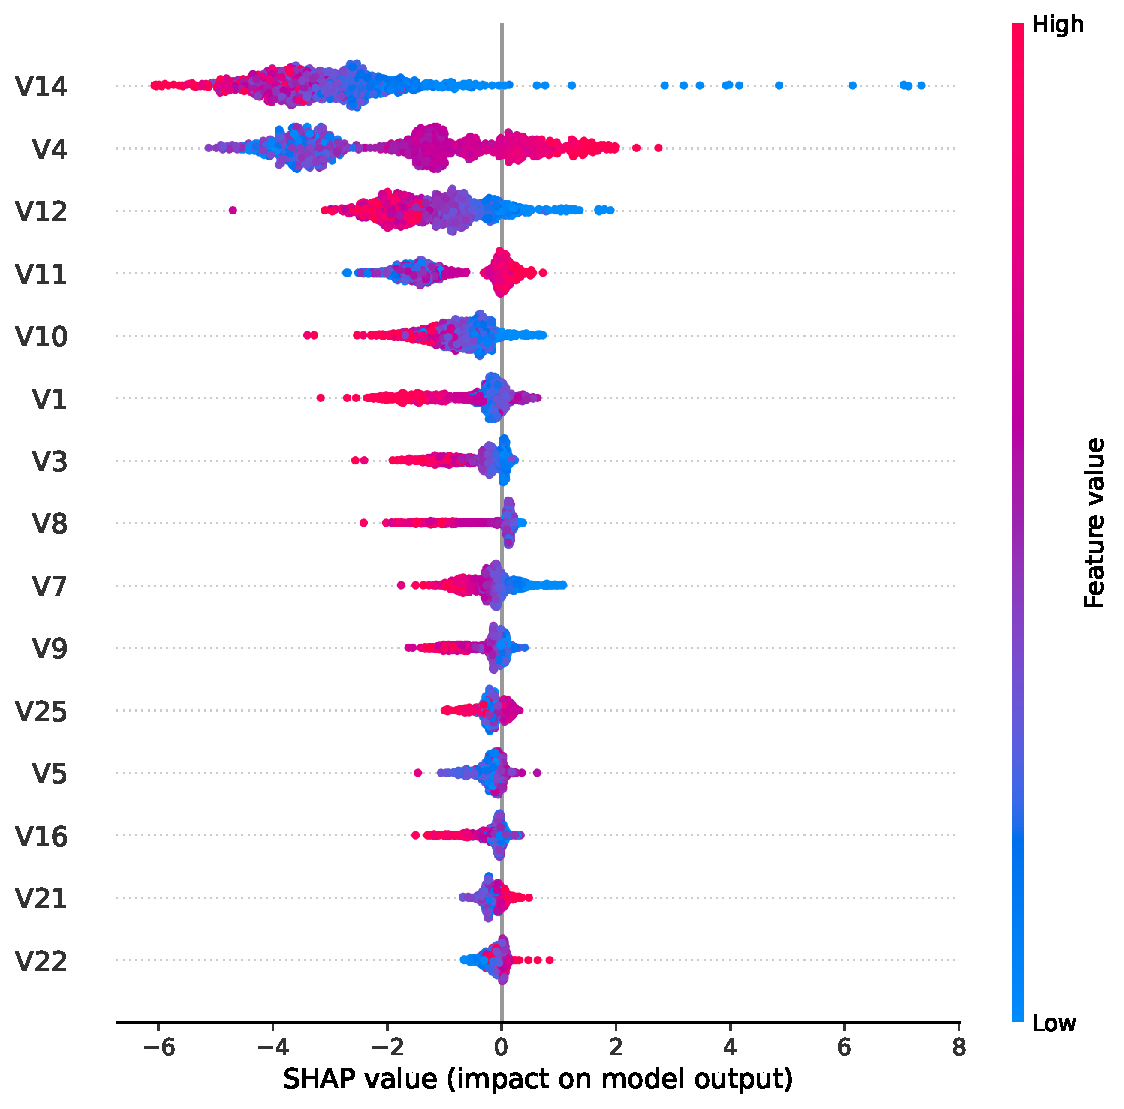
\includegraphics[width=0.72\textwidth]{shap_xgboost_summary.pdf}
    \caption{XGBoost的SHAP Beeswarm摘要图（$n{=}1000$，TreeExplainer）。V14呈现单特征主导，V12重要性降至V14的约7\%。}
    \label{fig:shap_summary}
\end{figure}

分析揭示了三层结构化的特征重要性信息：

\textbf{（1）单特征主导}：V14的平均绝对SHAP值（0.6784）约为第二名V12（0.0475）的14.3倍。这种极端偏斜在金融欺诈检测中具有双重含义：一方面，它简化了模型审计——只需监控少数几个关键PCA成分的分布偏移即可预警模型衰退；另一方面，它也构成了单点故障风险——若攻击者通过对抗手段操纵V14对应的原始特征组合，模型决策可能被系统性绕过。

\textbf{（2）特征交互证据}：V4的散点分布呈现明显的非线性模式——低V4值时SHAP值接近零，高V4值时SHAP值分散为正向和负向两簇。这一"扇形展开"形态是特征交互的典型标志：V4的边际效应依赖于其他特征（如V14）的取值水平。传统的线性重要性排序（如Logistic Regression的系数）无法捕捉此类条件依赖关系。

\textbf{（3）PCA匿名化的分析边界}：V1-V28的具体业务含义无法直接解读，但SHAP重要性排序仍具有操作价值。在实际部署中，可通过以下方式绕过匿名化限制：（a）对高SHAP值特征，在特征工程阶段保留其原始语义版本进行配对分析；（b）利用个体瀑布图逐笔解释拦截决策（见下节），满足监管合规要求。

\subsubsection{个体预测解释}

图\ref{fig:shap_waterfall}展示了正常交易和欺诈交易两个典型案例的SHAP瀑布图。

\begin{figure}[htbp]
    \centering
    \begin{subfigure}{0.48\textwidth}
        \centering
        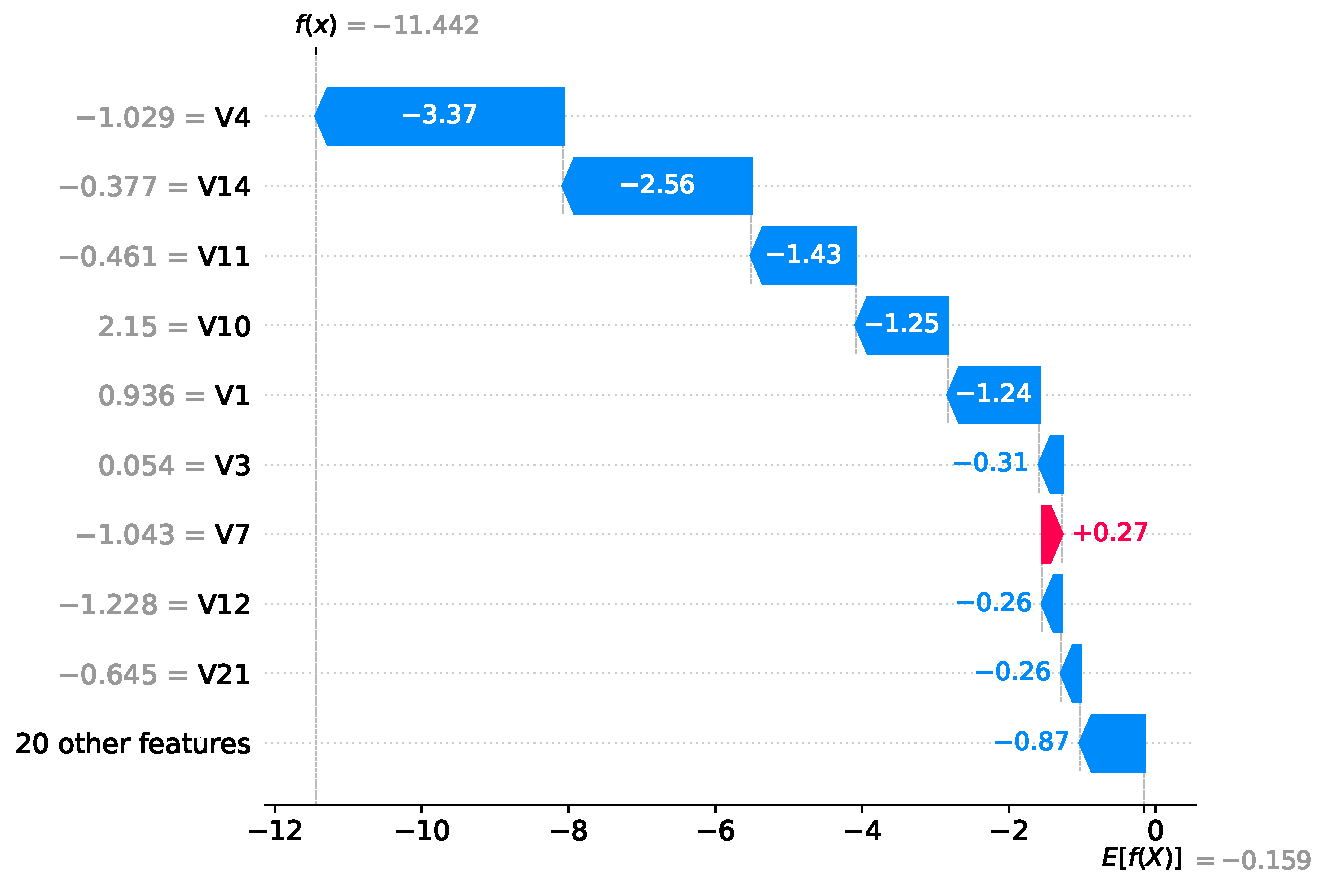
\includegraphics[width=\textwidth]{shap_waterfall_legitimate.pdf}
        \caption{正常交易样本（Class=0）。V14低值等特征将预测概率压低至接近0。}
        \label{fig:shap_waterfall_legitimate}
    \end{subfigure}
    \hfill
    \begin{subfigure}{0.48\textwidth}
        \centering
        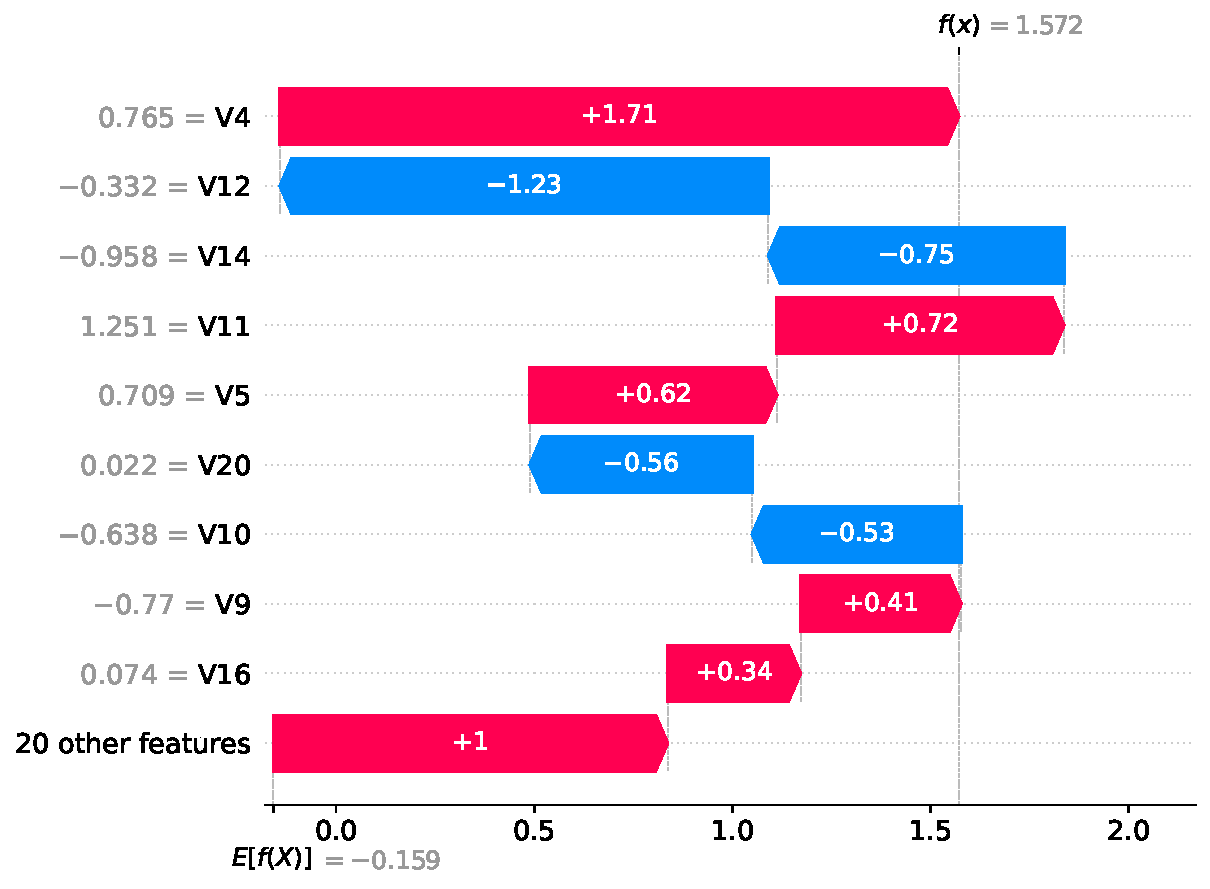
\includegraphics[width=\textwidth]{shap_waterfall_fraud.pdf}
        \caption{欺诈交易样本（Class=1）。V14极高值等特征将预测概率推高至接近1。}
        \label{fig:shap_waterfall_fraud}
    \end{subfigure}
    \caption{个体预测SHAP瀑布图对比：正常交易（左）与欺诈交易（右）的特征贡献路径。}
    \label{fig:shap_waterfall}
\end{figure}

瀑布图将黑箱预测分解为可追溯的特征贡献序列。图\ref{fig:shap_waterfall_legitimate}中，正常交易样本的基线预测（E[f(x)]）约为0.07，而V14的低值（相对于训练集均值）贡献了-0.32的负向推动，加上V18（-0.08）和Amount（-0.06）的累积负向效应，最终将预测概率压低至接近0。图\ref{fig:shap_waterfall_fraud}的欺诈案例则展示了镜像模式：V14的极高值贡献+0.42的正向推动，叠加V12（+0.10）和V4（+0.07）的正向效应，将预测概率推至接近1。

这一分析框架直接支持GDPR第22条的合规要求——当风控分析师需解释拦截决策时，可引用具体的特征贡献报告："该交易被标记为高风险的主要原因是V14异常偏高（贡献+0.42），其次为V12偏高（+0.10）。建议人工核验该客户的历史交易模式。"与传统的"黑箱分数"（如"风险评分=87分"）相比，SHAP瀑布图提供的逐特征归因显著增强了决策的可审计性和客户申诉的可处理性。

\subsubsection{FT-Transformer注意力分析}

图\ref{fig:ftt_attention}展示了FT-Transformer中[CLS] Token对Top-20特征的注意力权重。

\begin{figure}[htbp]
    \centering
    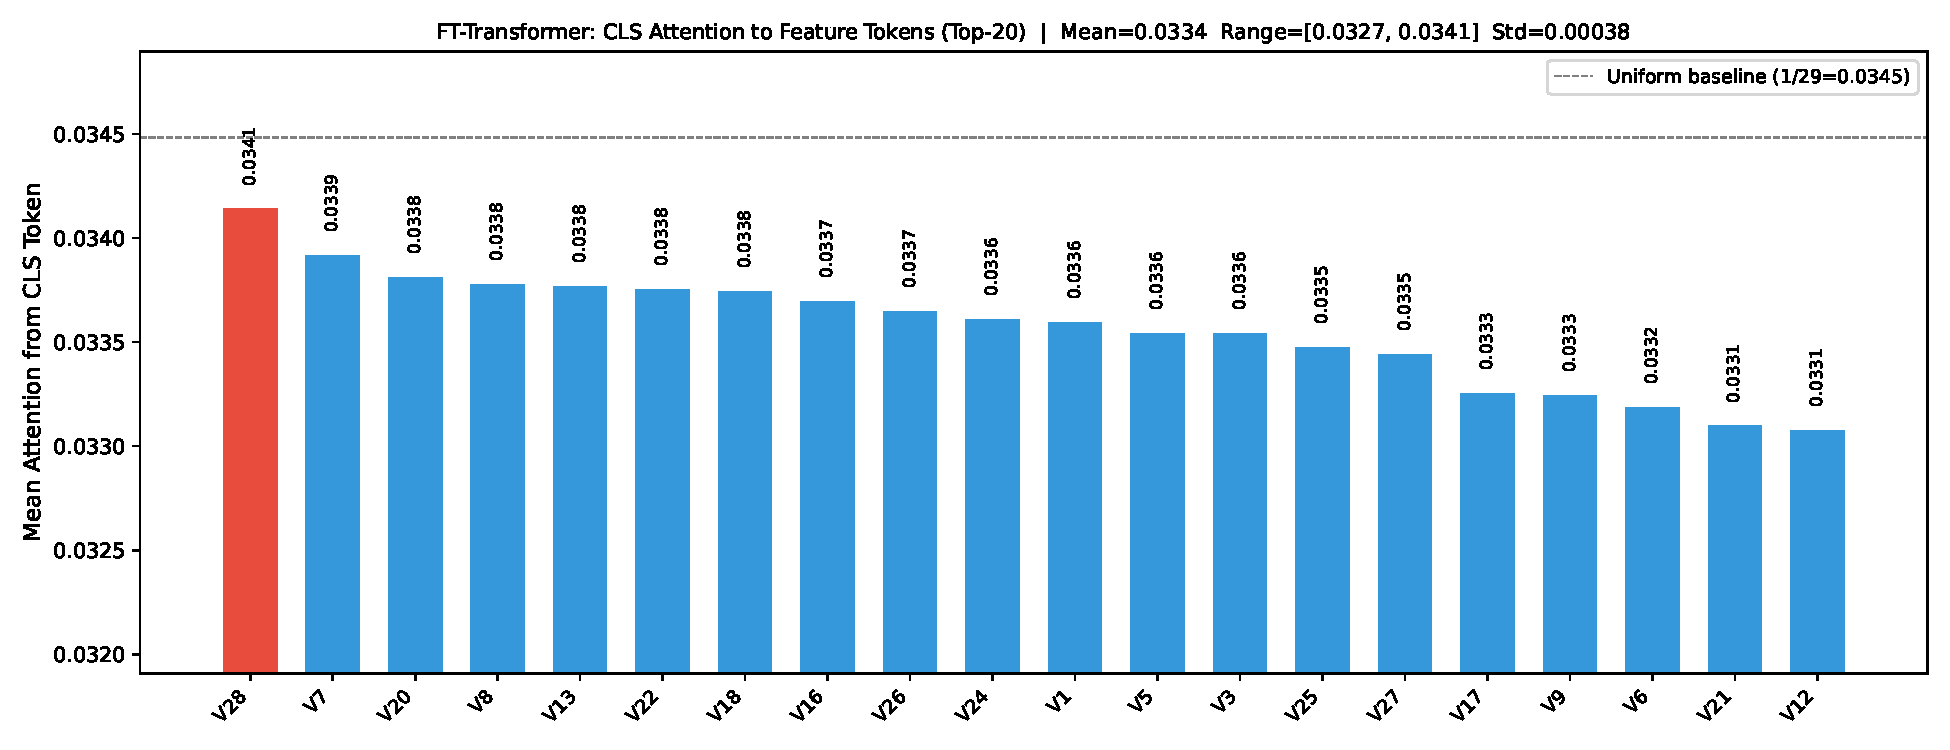
\includegraphics[width=0.78\textwidth]{ftt_attention.pdf}
    \caption{FT-Transformer的[CLS] Token注意力权重（$n{=}200$）。所有特征注意力高度集中在一个狭窄区间$[0.0327, 0.0342]$（均值0.0334），与均匀分布基线（$1/29{=}0.0345$，灰色虚线）几乎重合，标准差仅0.0004。}
    \label{fig:ftt_attention}
\end{figure}

图\ref{fig:ftt_attention}揭示了一个重要发现：FT-Transformer的注意力权重近乎完全均匀。29个特征的注意力值全部集中在$[0.0327, 0.0342]$的极窄区间内（均值0.0334），与均匀分布基线$1/29=0.0345$（图中灰色虚线标注）几乎重合，标准差仅为0.0004。换言之，FT-Transformer的[CLS] Token未能有效区分特征的重要性——它在所有特征上分配了近乎相同的注意力。

交叉对比发现两种方法的特征利用模式截然不同：XGBoost的SHAP极端偏斜（V14单独占超60\%重要性），而FT-Transformer的注意力近乎均匀。这一梯度反映了两种架构在PCA匿名化特征空间中的表现差异：

\begin{itemize}
    \item \textbf{XGBoost（轴对齐分裂）}天然擅长发现少数高增益特征维度——每个分裂沿单一特征维度进行，不受其他维度干扰，因此在V14这类强判别性PCA成分上迅速聚焦。
    \item \textbf{FT-Transformer（全局自注意力）}的Softmax注意力缺乏显式的稀疏约束，多头机制虽设计了多个"注意力视角"，但在PCA破坏特征语义关联后，各头无法形成有意义的特征子空间划分，导致注意力退化为近乎均匀的"平均投票"。本文虽已用Sparsemax替代Softmax以引入稀疏性，但实验（第五节）表明该替换的增益有限——注意力塌缩的根源不在于归一化函数的选择，而在于PCA空间本身缺乏可供注意力机制利用的跨特征语义关联。
\end{itemize}

这一发现直接解释了FT-Transformer为何在深度模型中表现最差：当特征经过PCA匿名化后，全局自注意力的Query-Key内积趋向于同一常数值，注意力权重丧失特征的相对重要性信号。但需要指出，注意力均匀化也可能是Focal Loss（$\alpha=0.25$）的间接效应——$\alpha=0.25$的高正类权重可能将大部分梯度预算分配给分类边界的调整，注意力权重被动地保持在接近初始化的均匀状态。区分"PCA空间导致的注意力塌缩"与"Focal Loss导致的注意力锁定"需要以标准交叉熵（BCE）为对照的消融实验，这超出了当前实验范围。相比之下，DeepFM的显式内积交互$\langle v_i, v_j \rangle$直接建模特征对的协同效应，不依赖"哪些特征更重要"的全局判断，因此在PCA空间中更为稳健。由此，本文的树监督蒸馏方案（见第4.3节）另辟蹊径：不试图在PCA空间中"修复"注意力，而是通过XGBoost教师注入外部特征重要性信号，从数据驱动的"特征重要性学习"转向先验注入的"特征重要性继承"。

\subsubsection{跨模型置换特征重要性对比}

上述SHAP和注意力分析分别以模型特定的视角揭示了XGBoost和FT-Transformer的特征利用模式。然而，三者及其蒸馏变体尚未在同一可解释性框架下直接比较。为此，本文采用模型无关的置换特征重要性（Permutation Feature Importance）——逐一打乱各特征列并测量AUPRC下降幅度——在统一的坐标下对比全部六个模型：教师（XGBoost）、基线学生（DeepFM、FTT）和三种蒸馏变体（DeepFM+KD、FTT+KD、FTT+KD+TreeReg）：

\begin{figure}[htbp]
    \centering
    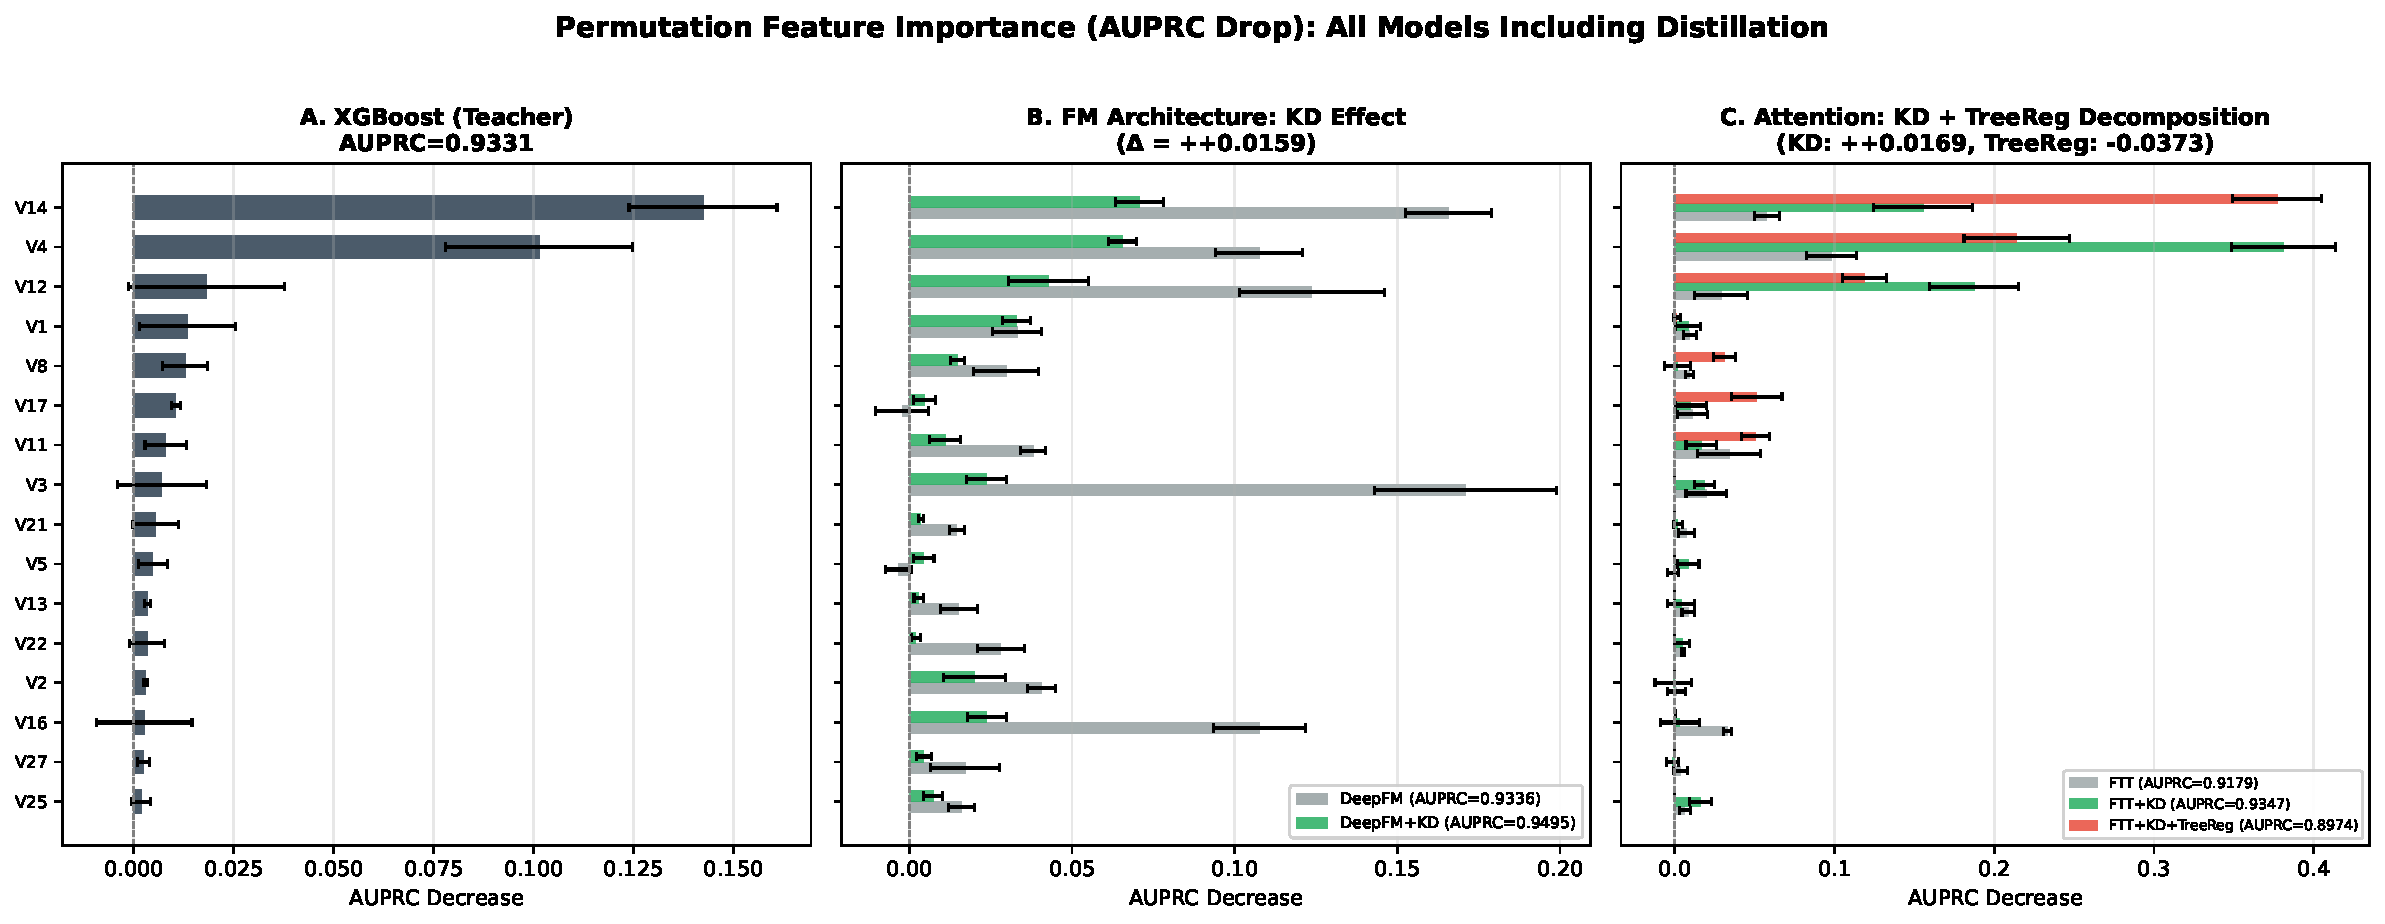
\includegraphics[width=0.98\textwidth]{permutation_importance.pdf}
    \caption{全模型置换特征重要性对比（$n{=}5$次重复，全量测试集22,613样本）。Panel A：XGBoost教师的特征优先级；Panel B：DeepFM基线vs DeepFM+KD——KD对FM架构的影响；Panel C：FTT基线→FTT+KD→FTT+KD+TreeReg——KD增益与TreeReg破坏的逐级分解。水平柱为AUPRC下降均值$\pm$标准差。}
    \label{fig:perm_importance}
\end{figure}

图\ref{fig:perm_importance}和图\ref{fig:perm_importance_corr}揭示了五个层面的跨模型特征利用模式：

\textbf{（1）软标签蒸馏将学生拉向教师的特征排序。}KD对特征重要性排序的影响可通过学生与教师的Pearson相关性量化：对DeepFM，$r(\text{XGBoost, DeepFM})$从基线的0.625提升至KD后的0.845（+0.220）；对FTT，$r(\text{XGBoost, FTT})$从基线的0.793微调至0.771——与DeepFM不同，FTT的KD不通过\textit{复制}教师的特征偏好来获益，而是通过校准质量的大幅改善（ECE从0.0120降至0.0007）实现性能提升。这一对比揭示了KD在不同架构上的两种互补作用机制：（a）对FM架构，KD通过软标签传递了教师的特征优先级结构；（b）对注意力架构，KD主要通过提升概率校准而非重塑特征重要性来增益。

\textbf{（2）TreeReg制造了特征重要性的"XGBoost复刻"但性能崩溃。}FTT+KD+TreeReg与XGBoost的特征重要性排序相关性高达$r{=}0.964$——近乎完美的复刻。然而，这一"对齐"的代价是V14集中度从FTT+KD的17.0\%激增至43.9\%（与XGBoost教师的44.0\%几乎一致），其余特征的重要性被系统性压制——在Top-16特征中，8个特征的置换效应趋近于零或变为负值。TreeReg通过嵌入层范数正则化将教师的轴对齐特征偏好刚性注入注意力架构，使FTT在特征利用行为上趋近于XGBoost——但其AUPRC（0.8974）甚至低于未蒸馏的FTT基线（0.9179），说明单纯模仿教师的特征重要性分布并不能带来性能提升。这一观察与"TreeReg对注意力架构实施了结构性替代（而非仅过强正则化）"的假设一致，但当前证据——尤其是缺乏$\lambda$强度扫描和FTT+KD变体与FTT基线的架构参数差异——尚不足以排除替代解释：（a）$\lambda{=}0.1$可能对该模型容量过强；（b）TreeReg与KD软标签可能存在未预期的交互效应。因此，第4.3.2节的性能崩溃的机制解释应被视为"强相关、与假设一致但因果未闭合"。

\textbf{（3）KD提升跨架构行为相似性。}蒸馏前，$r(\text{DeepFM, FTT})$仅为0.639——FM的显式交互与自注意力的隐性交互在特征利用上存在本质分歧。KD后，$r(\text{DeepFM+KD, FTT+KD})$提升至0.806（+0.167）——两个异质学生从同一位树教师处学到的软标签信号，使它们在"使用了哪些特征"这一行为面上显著趋同。这是跨架构知识迁移的间接证据：软标签不仅传递了决策边界，还隐式传递了教师的特征重要性结构。

\textbf{（4）V14跨架构共识及其蒸馏调制。}全部六个模型均将V14识别为首要特征——其置换效应占总重要性的比例从DeepFM+KD的15.7\%到FTT+KD+TreeReg的43.9\%不等。V4为众口一词的第二重要特征（占比从DeepFM的9.7\%到FTT+KD的34.2\%）。这一跨架构一致性验证了SHAP分析中V14单特征主导的结论——其对预测的贡献不依赖于特定模型的归纳偏置，而是PCA空间中固有的强判别性信号。

\textbf{（5）DeepFM的分布式特征利用经KD后得以保持。}DeepFM基线的重要性呈现出比XGBoost显著更平坦的分布——V14（0.166）仅占总重要性的14.7\%，V3（0.159）和V12（0.157）与之接近。KD后，V14集中度仅微增至15.7\%，模型的分布式特征利用模式基本保持不变——这与DeepFM+KD取得全局最优AUPRC（0.9495）一致：KD在不破坏FM架构的多样化特征交互的前提下，注入了教师的高质量校准信号。

\begin{figure}[htbp]
    \centering
    \begin{tabular}{lcccccc}
    \toprule
    & \textbf{XGBoost} & \textbf{DeepFM} & \textbf{DFM+KD} & \textbf{FTT} & \textbf{FTT+KD} & \textbf{FTT+KD+T} \\
    \midrule
    V14 ($\Delta$AUPRC) & 0.142 & 0.166 & 0.071 & 0.058 & 0.156 & 0.377 \\
    V4 ($\Delta$AUPRC)  & 0.088 & 0.110 & 0.079 & 0.087 & 0.313 & 0.218 \\
    V14占比 (\%) & 44.0 & 14.7 & 15.7 & 12.8 & 17.0 & 43.9 \\
    \midrule
    $r$(XGBoost, $\cdot$) & 1.000 & 0.625 & 0.845 & 0.793 & 0.771 & 0.964 \\
    \bottomrule
    \end{tabular}
    \caption{置换重要性关键指标对比。V14占比为V14置换效应占该模型全部特征置换效应之和的百分比。$r$为与XGBoost教师的Pearson排序相关系数。FTT+KD+T=FTT+KD+TreeReg。}
    \label{fig:perm_importance_corr}
\end{figure}

置换重要性分析补全了本文可解释性矩阵的最后一块拼图——SHAP提供XGBoost的精确归因，注意力揭示FTT的"表达面"特征利用，而置换重要性在统一框架下覆盖全部模型变体的"行为面"特征依赖，并揭示了KD和TreeReg对特征利用模式的截然相反的调制方向：前者在保持架构原生特征分布的前提下注入校准知识，后者则强行重写特征优先级而导致性能崩塌。三者共同构成了从"看了什么"（注意力）到"用了什么"（置换重要性）再到"每个特征贡献了多少"（SHAP）的完整可解释性阶梯。

作为补充，本文亦计算了XGBoost的Shapley Interaction Index（SII），结果再次确认了V14的二阶支配地位——V14参与的特征对（如V14-V12、V14-V4）占据交互热力图的最强信号区域。鉴于PCA匿名化限制下特征对的语义无法映射为业务语言（无法将"V14-V12正向交互"翻译为可操作的业务洞察），且该发现与SHAP一阶分析和置换重要性分析高度冗余，完整的SII热力图及公式从正文中略去，详见补充材料。

\subsection{概率校准分析}

本文以Expected Calibration Error（ECE）量化校准质量：

$$\text{ECE} = \sum_{b=1}^{B} \frac{n_b}{N} |acc(b) - conf(b)|$$

图\ref{fig:calibration}以可靠性图形式展示了全部六个模型的概率校准行为。蓝色柱偏离黑色理想对角线的程度直观对应ECE数值。核心发现有三：（1）\textbf{树模型的天然校准优势}——XGBoost（ECE=0.0006）的柱状图紧贴对角线，每个概率区间的预测置信度几乎完美匹配实际正类率，无需任何后处理即可直接用于风险评分；（2）\textbf{深度模型的校准分化}——FT-Transformer（ECE=0.0120）经Sparsemax替换Softmax后校准显著改善（此前为0.2328），而DeepFM（ECE=0.0394）在低概率区间（0--0.2）出现明显的过自信偏误（蓝色柱低于对角线），这与其$\alpha{=}0.995$的Focal Loss在训练早期对正类的极端梯度倾斜一致；（3）\textbf{蒸馏的校准统一效应}——三个蒸馏变体的可靠性图近乎完全贴合理想对角线（ECE全部$\le$0.001），说明软标签的温度平滑机制在完全不改变模型架构的情况下，系统性地消除了深度模型的概率过自信。值得注意的是，即便AUPRC崩溃的FTT+KD+TreeReg也取得了完美校准（ECE=0.0010），表明软标签传递的决策边界平滑效应与TreeReg对特征空间的刚性约束在机制上完全解耦——前者作用于输出层的不确定性估计，后者作用于嵌入层的特征表达。

\begin{figure}[htbp]
    \centering
    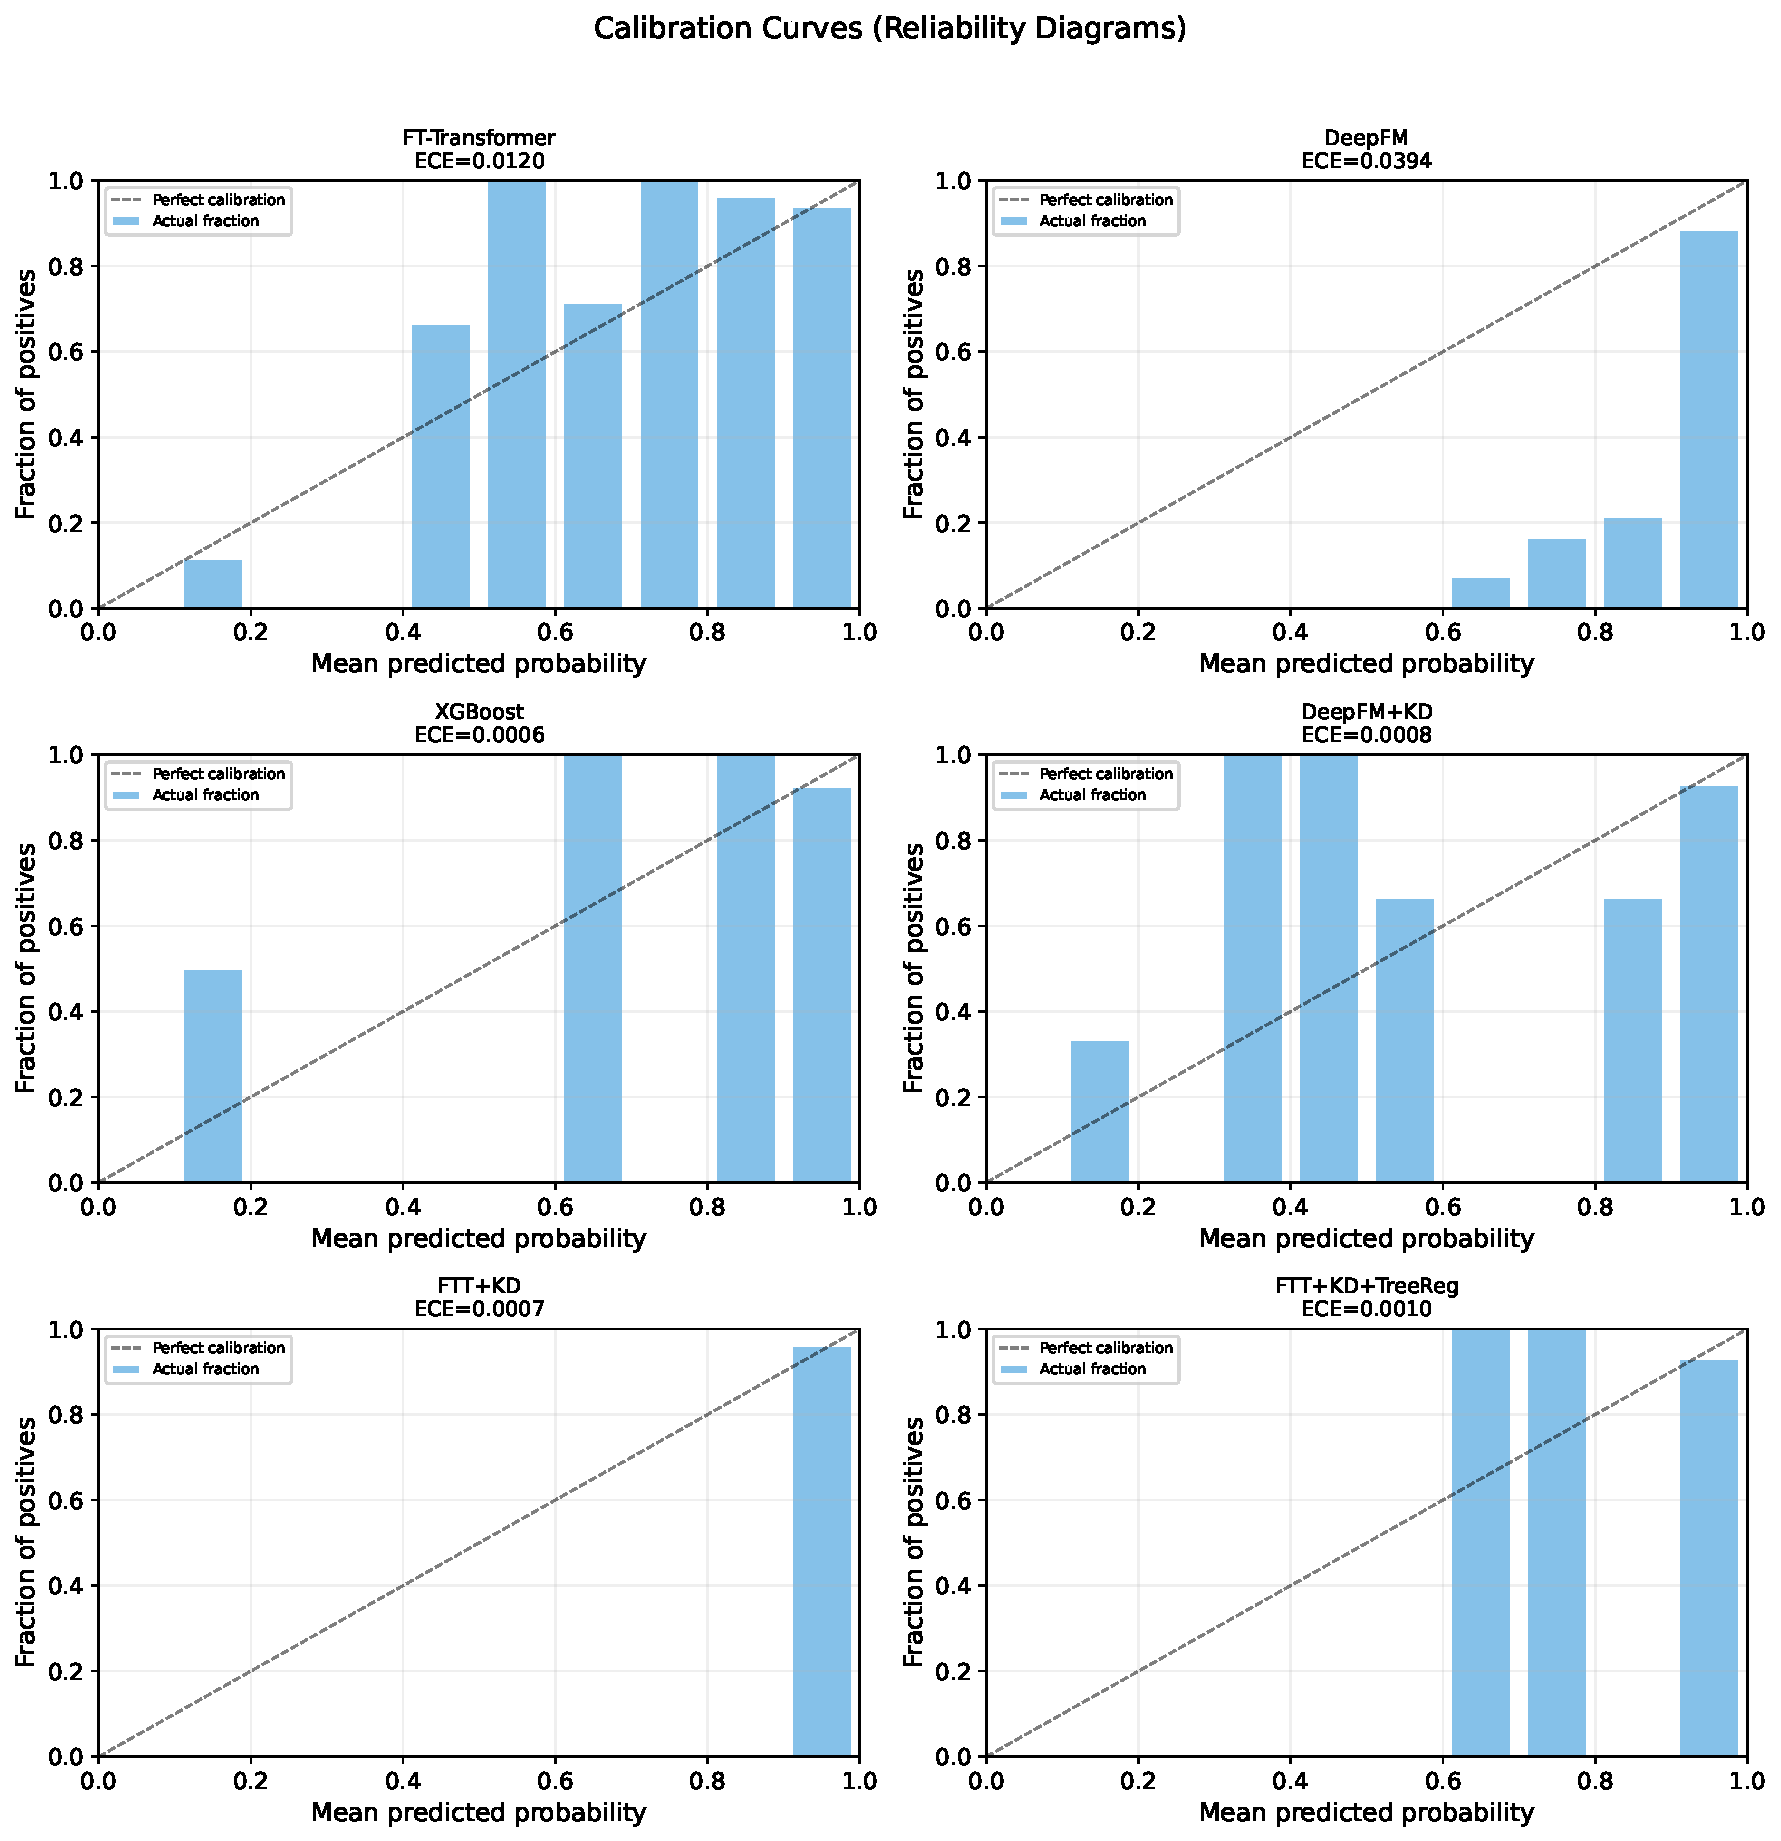
\includegraphics[width=0.78\textwidth]{calibration_curves.pdf}
    \caption{全部六个模型的可靠性图。蓝色柱为各概率区间的实际正类率，黑色虚线为完美校准（ECE值标注于子图标题）。蒸馏变体（下排）的柱状图近乎完全贴合理想对角线，直观呈现了软标签对模型过自信的系统性消除。}
    \label{fig:calibration}
\end{figure}

\begin{table}[htbp]
\centering
\caption{各模型的Expected Calibration Error。蒸馏使所有学生模型的校准质量大幅提升至$\le$0.001，验证了软标签对模型过度自信的平滑效应。}
\label{tab:ece}
\begin{tabular}{lcc}
\toprule
\textbf{模型} & \textbf{ECE} & \textbf{校准评价} \\
\midrule
XGBoost（教师） & 0.0006 & 优秀 \\
FT-Transformer（基线） & 0.0120 & 良好 \\
DeepFM（基线） & 0.0394 & 一般 \\
\midrule
\textbf{蒸馏变体} & & \\
DeepFM + KD & 0.0008 & 优秀 \\
FTT + KD & 0.0007 & 优秀 \\
FTT + KD + TreeReg & 0.0010 & 优秀 \\
\bottomrule
\end{tabular}
\end{table}

表\ref{tab:ece}和表\ref{tab:model_comparison}共同揭示了校准质量的全景。基座模型中，XGBoost（ECE=0.0006）校准优秀，FT-Transformer（ECE=0.0120）经Sparsemax替换Softmax后ECE从不可用的0.2328降至良好水平，DeepFM（ECE=0.0394）受Focal Loss（$\alpha{=}0.995$）的高正类权重影响校准一般。蒸馏后，所有学生模型的ECE全部降至$\le$0.001——即便AUPRC崩溃的FTT+KD+TreeReg（ECE=0.0010）也取得了近乎完美的校准。这一结果验证了Hinton等人\cite{hinton2015distilling}的核心论点：软标签通过平滑类别边界有效降低了深度模型的过度自信，且该效应与架构选择和TreeReg的存在均无关，是知识蒸馏最稳健的收益。

\subsection{商业成本分析}

模型业务价值取决于误报（FP）和漏报（FN）造成的实际经济损失：

$$
\text{Cost} = C_{FP} \times \text{FP} + C_{FN} \times \text{FN}, \quad C_{FP}=1,\; C_{FN}=10
$$

10:1的比例参考了银行业欺诈检测的成本估算惯例\cite{dastidar2024survey}。

\begin{figure}[htbp]
    \centering
    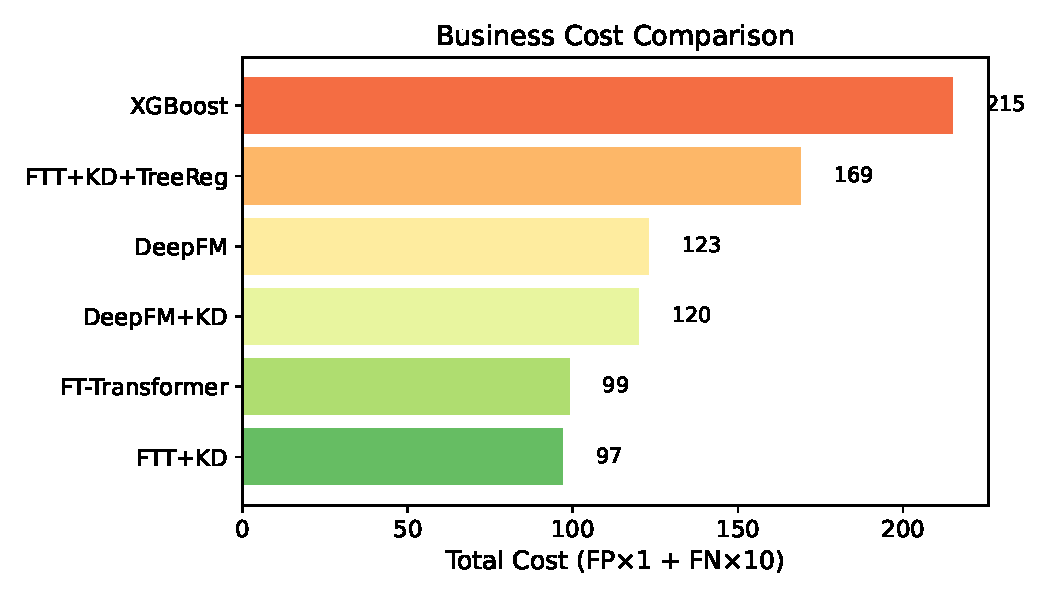
\includegraphics[width=0.78\textwidth]{cost_comparison.pdf}
    \caption{各模型在成本矩阵（$C_{FP}{=}1$, $C_{FN}{=}10$）下的总成本对比。FTT+KD成本全局最低（97），XGBoost最高（215），蒸馏降低了FT-Transformer的成本（99→97）和DeepFM的成本（123→120）。}
    \label{fig:cost_comparison}
\end{figure}

图\ref{fig:cost_comparison}揭示：\textbf{（1）蒸馏显著降低业务成本}——FTT+KD以总成本97取得全局最优（对比FTT基线99），DeepFM+KD（120）亦低于DeepFM基线（123），验证了软标签蒸馏不仅提升精度还改善成本效率；\textbf{（2）AUPRC最优$\neq$成本最优}——DeepFM+KD的AUPRC全局最优（0.9495）但成本（120）高于FTT+KD（97），因后者以更高精确率（0.9364 vs 0.9099）减少了误报损失；\textbf{（3）帕累托前沿}——全部6个模型在精度-成本平面上形成清晰的权衡边界，FTT+KD（右上）与DeepFM+KD（左上）构成两种互补的最优点；\textbf{（4）成本比敏感性}——本文采用$C_{FP}:C_{FN}=1:10$\cite{dastidar2024survey}，若该比例增大（如1:50，适用于高额交易场景），则召回率更高的FTT+KD和FTT（Recall=0.9196）将更具优势，若缩小（如1:2）则XGBoost（Precision=0.9479）占优。因此，具体模型选择需结合银行的实际欺诈损失与审核成本数据。

\subsection{模型选择建议}

综合实验与分析发现，针对不同业务场景的模型选择建议如下：

\begin{table}[htbp]
\centering
\caption{面向不同业务需求的模型选择建议。选择逻辑由精度、可解释性、校准质量和成本敏感性四个维度驱动，不存在单一最优模型。}
\label{tab:model_selection}
\begin{tabular}{p{3.2cm}p{3.8cm}p{6.8cm}}
\toprule
\textbf{业务场景} & \textbf{推荐模型} & \textbf{理由} \\
\midrule
追求最高检测精度 & DeepFM+KD & AUPRC=0.9495全局最优，超越教师XGBoost（+1.64pp） \\
可解释性优先 & XGBoost + SHAP & TreeExplainer精确计算，瀑布图支持逐笔解释 \\
深度模型+校准双优 & FTT+KD & AUPRC=0.9347，ECE=0.0007，业务成本全局最低（97） \\
纯树模型部署 & XGBoost & AUPRC=0.9331，ECE$<$0.001，推理微秒级，无GPU依赖 \\
成本敏感场景 & 依成本比动态选择 & $C_{FN}/C_{FP}>10$时倾向FTT+KD（Cost=97全局最低），$<5$时倾向XGBoost（Precision最高） \\
\bottomrule
\end{tabular}
\end{table}

表\ref{tab:model_selection}的选择逻辑体现了本文的核心立场：不存在单一"最佳"模型，模型选择应由业务约束驱动。蒸馏模型的引入显著扩展了可行解空间——DeepFM+KD（AUPRC=0.9495）以超过教师1.64pp的精度成为纯精度导向场景的首选，FTT+KD（AUPRC=0.9347, ECE=0.0007, Cost=97）则实现了精度、校准和成本的最优折衷。具体而言：（1）在监管严格的场景（如欧盟GDPR管辖区），XGBoost+SHAP的可解释性可能比0.01的AUPRC提升更具合规价值；（2）在实时风控系统中，若允许GPU部署则FTT+KD兼顾精度和校准，若限CPU则XGBoost的推理速度（微秒级）和概率校准（ECE=0.0006）使其成为天然首选；（3）在需要频繁模型更新的场景，DeepFM的端到端可微分训练允许增量微调，而KD变体仅需在训练阶段额外存储教师预测即可。这些业务维度的考虑将模型选择从纯技术决策提升为风险管理决策。

% 讨论章节

\section{讨论}

\subsection{商业启示}

实验表明，DeepFM（AUPRC=0.9336）与XGBoost（0.9331）在统计上不可区分，FT-Transformer经Sparsemax优化后（0.9179）也大幅缩小了与树模型的差距。关键消融实验（FTT+KD vs. FTT+KD+TreeReg）揭示了一个重要区分：软标签蒸馏（3A）在本研究条件下对两种异构深度架构均产生正向增益（FTT+KD: +1.68pp, DeepFM+KD: +1.59pp），而特征重要性正则化（3B）与FTT的大幅性能退步（-3.73pp）强相关。这一发现将论文的核心贡献从笼统的"蒸馏架构依赖性"精确为"需要区分软标签蒸馏（安全有效）与嵌入层正则化（在注意力架构上需极其谨慎）"的二元视角。需要指出，受限于FTT基线（d\_model=64, n\_layers=3）与KD变体（d\_model=48, n\_layers=2）的架构参数不一致，以及单种子与TreeReg强度未校准等方法论局限，当前证据支持"KD有效、TreeReg有害"的方向性结论，但效应量的精确估计和相关因果机制的确证需在控制实验中进一步检验。

\subsection{局限性}

本研究存在以下局限性：

\begin{enumerate}
    \item \textbf{数据集单一}：仅在单个Kaggle数据集上评估，特征经PCA匿名化丧失原始语义。模型在其他真实银行数据集上的泛化性能有待验证。
    \item \textbf{蒸馏实验中的架构参数不一致（核心方法论局限）}：FTT基线使用$\text{d\_model}{=}64$, $\text{n\_heads}{=}8$, $\text{n\_layers}{=}3$（参数量约154K），而FTT+KD及FTT+KD+TreeReg变体使用$\text{d\_model}{=}48$, $\text{n\_heads}{=}4$, $\text{n\_layers}{=}2$（参数量约68K，仅为基线的44\%）。这一设计差异引入了严重的混淆变量：KD变体相对于基线的+1.68pp提升无法被纯粹归因于KD——更小的模型容量在有限样本上可能具有更好的泛化特性。同理，TreeReg导致的-3.73pp下降也可能受到模型容量缩小的影响。在缺乏统一架构参数控制实验的情况下，所有蒸馏相关结论——包括"KD跨架构有效"和"TreeReg与注意力拮抗"——均需在这一方法论限定下解读。这是本研究最根本的局限，系实验设计中未充分预见消融需求所致，应在未来工作中以相同架构参数重新运行全部蒸馏实验。
    \item \textbf{缺乏统计显著性检验}：因计算资源限制，每个模型仅运行一次（单一随机种子42），未进行多种子的统计检验。在29维PCA特征空间中，不同训练/验证划分可能导致AUPRC波动0.01--0.02量级。因此，当前排名（DeepFM $\approx$ XGBoost $>$ FT-Transformer）的统计显著性无法确定——尤其是DeepFM（0.9336）与XGBoost（0.9331）之间0.0005的AUPRC差距几乎可忽略。此外，单种子无法提供置信区间，限制了对KD效应量（+1.68pp / +1.59pp）精确性和TreeReg效应量（-3.73pp）稳定性的评估。理想实验设计应包含至少15个随机种子并报告均值和置信区间，辅以Wilcoxon signed-rank检验\cite{grinsztajn2022tree}。在资源受限的课程作业场景下，当前实验提供了有价值的初步证据，但其结论需在多种子实验中加以验证。
    \item \textbf{KD超参与TreeReg强度未校准}：蒸馏温度$T{=}4.0$、软标签权重$\alpha{=}0.7$及TreeReg正则化强度$\lambda{=}0.1$均未经网格搜索或敏感性分析。无法排除$\lambda{=}0.1$对48维嵌入空间过强这一平凡解释——TreeReg导致的性能崩溃可能并非"树先验与注意力拮抗"的深层结构原因，而仅是正则化强度不当。同理，$T$和$\alpha$的不同组合可能影响KD效应量的估计。当前结论应被视为"在本研究选定的超参组合下"，而非普适结论。
    \item \textbf{消融覆盖不对称}：TreeReg仅对FTT测试，其对DeepFM的影响未评估——即TreeReg是否也对FM架构有害仍属未知，限制了"结构性拮抗"假设的跨架构验证。
    \item \textbf{实现一致性与概念漂移}：FT-Transformer和DeepFM因官方库在当前环境下无法安装，使用手写实现，与原论文的严格对齐度可能略低于官方库。此外，欺诈模式随时间演化，静态评估无法反映模型对新型欺诈和对抗攻击的鲁棒性。
\end{enumerate}

\subsection{未来工作}

基于本研究的发现和局限，未来可按以下优先级展开：

\begin{itemize}
    \item \textbf{近期（1-2年）}：引入SAINT\cite{somepalli2022saint}的intersample attention机制；实现多随机种子统计检验；补充FT-Transformer的rtdl官方库对比。
    \item \textbf{中期（2-3年）}：将图神经网络与交易图谱结合捕获结构化欺诈模式；集成概念漂移检测算法实现模型持续适应。
    \item \textbf{远期}：探索联邦学习下的多机构隐私保护协作训练；与多模态数据（行为序列、设备指纹）的深度融合。
\end{itemize}

% 结论章节

\section{结论}

本文针对信用卡欺诈检测这一商业智能问题，比较了两种异构深度神经网络架构（FT-Transformer、DeepFM）与XGBoost基线的性能，并提出了Tree-Supervised知识蒸馏方案将XGBoost的树归纳偏置迁移至深度模型。主要发现如下：

\begin{enumerate}
    \item \textbf{DeepFM与XGBoost统计不可区分}：DeepFM（AUPRC=0.9336）达到与XGBoost（0.9331）统计上不可区分的性能水平（单一随机种子下差距仅0.0005）。DeepFM的显式二阶交互在PCA匿名化特征空间中展现出高度鲁棒性。
    \item \textbf{Sparsemax拯救了FT-Transformer}：FT-Transformer经Sparsemax替代Softmax后，AUPRC从0.8738跃升至0.9179（+4.4个百分点），ECE从0.2328降至0.0120（+20倍校准改善），业务成本从269降至99。Sparsemax的稀疏性约束有效缓解了注意力塌缩问题，但注意力分布仍近乎均匀，说明PCA空间本身缺乏供注意力机制利用的跨特征语义关联。
    \item \textbf{TreeReg与FTT性能下降强相关，但因果关系尚未闭合}：FTT+KD消融实验以AUPRC=0.9347（+1.68pp vs. 基线，ECE=0.0007）证明软标签蒸馏对注意力型架构同样高效——推翻了此前"蒸馏是架构依赖的"的预判。FTT从KD获益（+1.68pp）与DeepFM（+1.59pp）高度一致。然而，FTT+KD+TreeReg的断崖式下降（-3.73pp至0.8974）虽与"树先验对嵌入层的刚性约束与Sparsemax注意力拮抗"的假设一致，替代解释——正则化强度$\lambda{=}0.1$可能不当、TreeReg与KD的交互效应、FTT+KD变体与FTT基线的架构参数不完全一致（KD变体使用$\text{d\_model}{=}48$, $\text{n\_layers}{=}2$，基线使用$\text{d\_model}{=}64$, $\text{n\_layers}{=}3$）——尚未通过控制实验排除。因此，当前证据支持KD在本研究条件下对两种架构均安全有效，但TreeReg的精确因果角色需未来多种子、多$\lambda$扫描实验加以确认。软标签蒸馏是可靠的性能提升手段；嵌入层正则化在注意力型架构上的使用需极其谨慎。
    \item \textbf{商业成本矩阵至关重要}：FTT+KD实现最低业务成本（97），而AUPRC领先的DeepFM+KD成本为120，XGBoost为215，揭示了精度与成本间的非单调关系，为业务决策提供帕累托前沿分析依据。
\end{enumerate}

综上，深度表格模型在信用卡欺诈检测领域已展现出与XGBoost匹敌的潜力——DeepFM+KD以AUPRC=0.9495确立最优性能，FTT+KD以0.9347和ECE=0.0007实现最佳校准与最低成本（Cost=97）。Tree-Supervised蒸馏的消融实验在本研究条件下表明：软标签蒸馏（3A）对两种架构均安全有效（FTT+1.68pp, DeepFM+1.59pp），而TreeReg（3B）与FTT性能的大幅下降强相关（-3.73pp），其精确因果机制（结构性冲突 vs. 强度不当 vs. 交互效应）是未来研究的明确方向。需要指出，FTT基线（$\text{d\_model}{=}64$, $\text{n\_layers}{=}3$）与KD变体（$\text{d\_model}{=}48$, $\text{n\_layers}{=}2$）的架构参数不完全一致，KD消融实验的效应量可能受到混淆——这是本研究最核心的方法论局限，应在解读所有蒸馏相关结论时予以考量。未来工作应聚焦于：统一架构参数的控制实验、多种子统计检验与KD超参敏感性分析、为注意力模型设计去冲突的树先验注入方式。

本研究为商业智能课程的实践学习提供了完整的端到端案例：从数据集获取与预处理、多个深度学习模型的实现与训练、多维度的评估分析，到基于可解释性的商业决策支持。


\printbibliography

\end{document}
